\chapter{Resultados}

A fin de conocer el comportamiento del nivel del mar en la bahía durante las fáses cálidas y frías del ENSO, se grafican las sobrelevaciones mensuales junto a las franjas rojas que marcan la ocurrencia de un evento Niño y los descensos mensuales junto a las franjas azules que delimitan los meses dónde hubo evento Niña (Fig. \ref{fig:s_d_ENSOS}). En la parte superior puede notarse que las sobrelevaciones  mensuales tienen valores máximos que coinciden, en su mayoría, con los meses dónde ocurrió un fenómeno Niño (mes Niño). Se resaltan las sobrelevaciones de hasta 35 cm durante El Niño de 1982-1983 y las sobrelevaciones de 30 cm durante el Niño 1997-1998. Ambos eventos fueron clasificados bajo el criterio del índice ONI en la categoría \textit{muy fuerte} \footnote{Esto se puede consultar en la página web \url{https://ggweather.com/enso/oni.htm}}. De forma análoga a las sobrelevaciones, los descensos mensuales más acentuados se vieron en los meses Niña, resaltando los que se presentaron en 1955-1956 durante un evento Niña de categoría \textit{moderada} y en 2007-2008 durante un evento de categoría \textit{fuerte}, fueron de -35 cm y -40 cm respectivamene.

\begin{figure}[H]
	\centering
	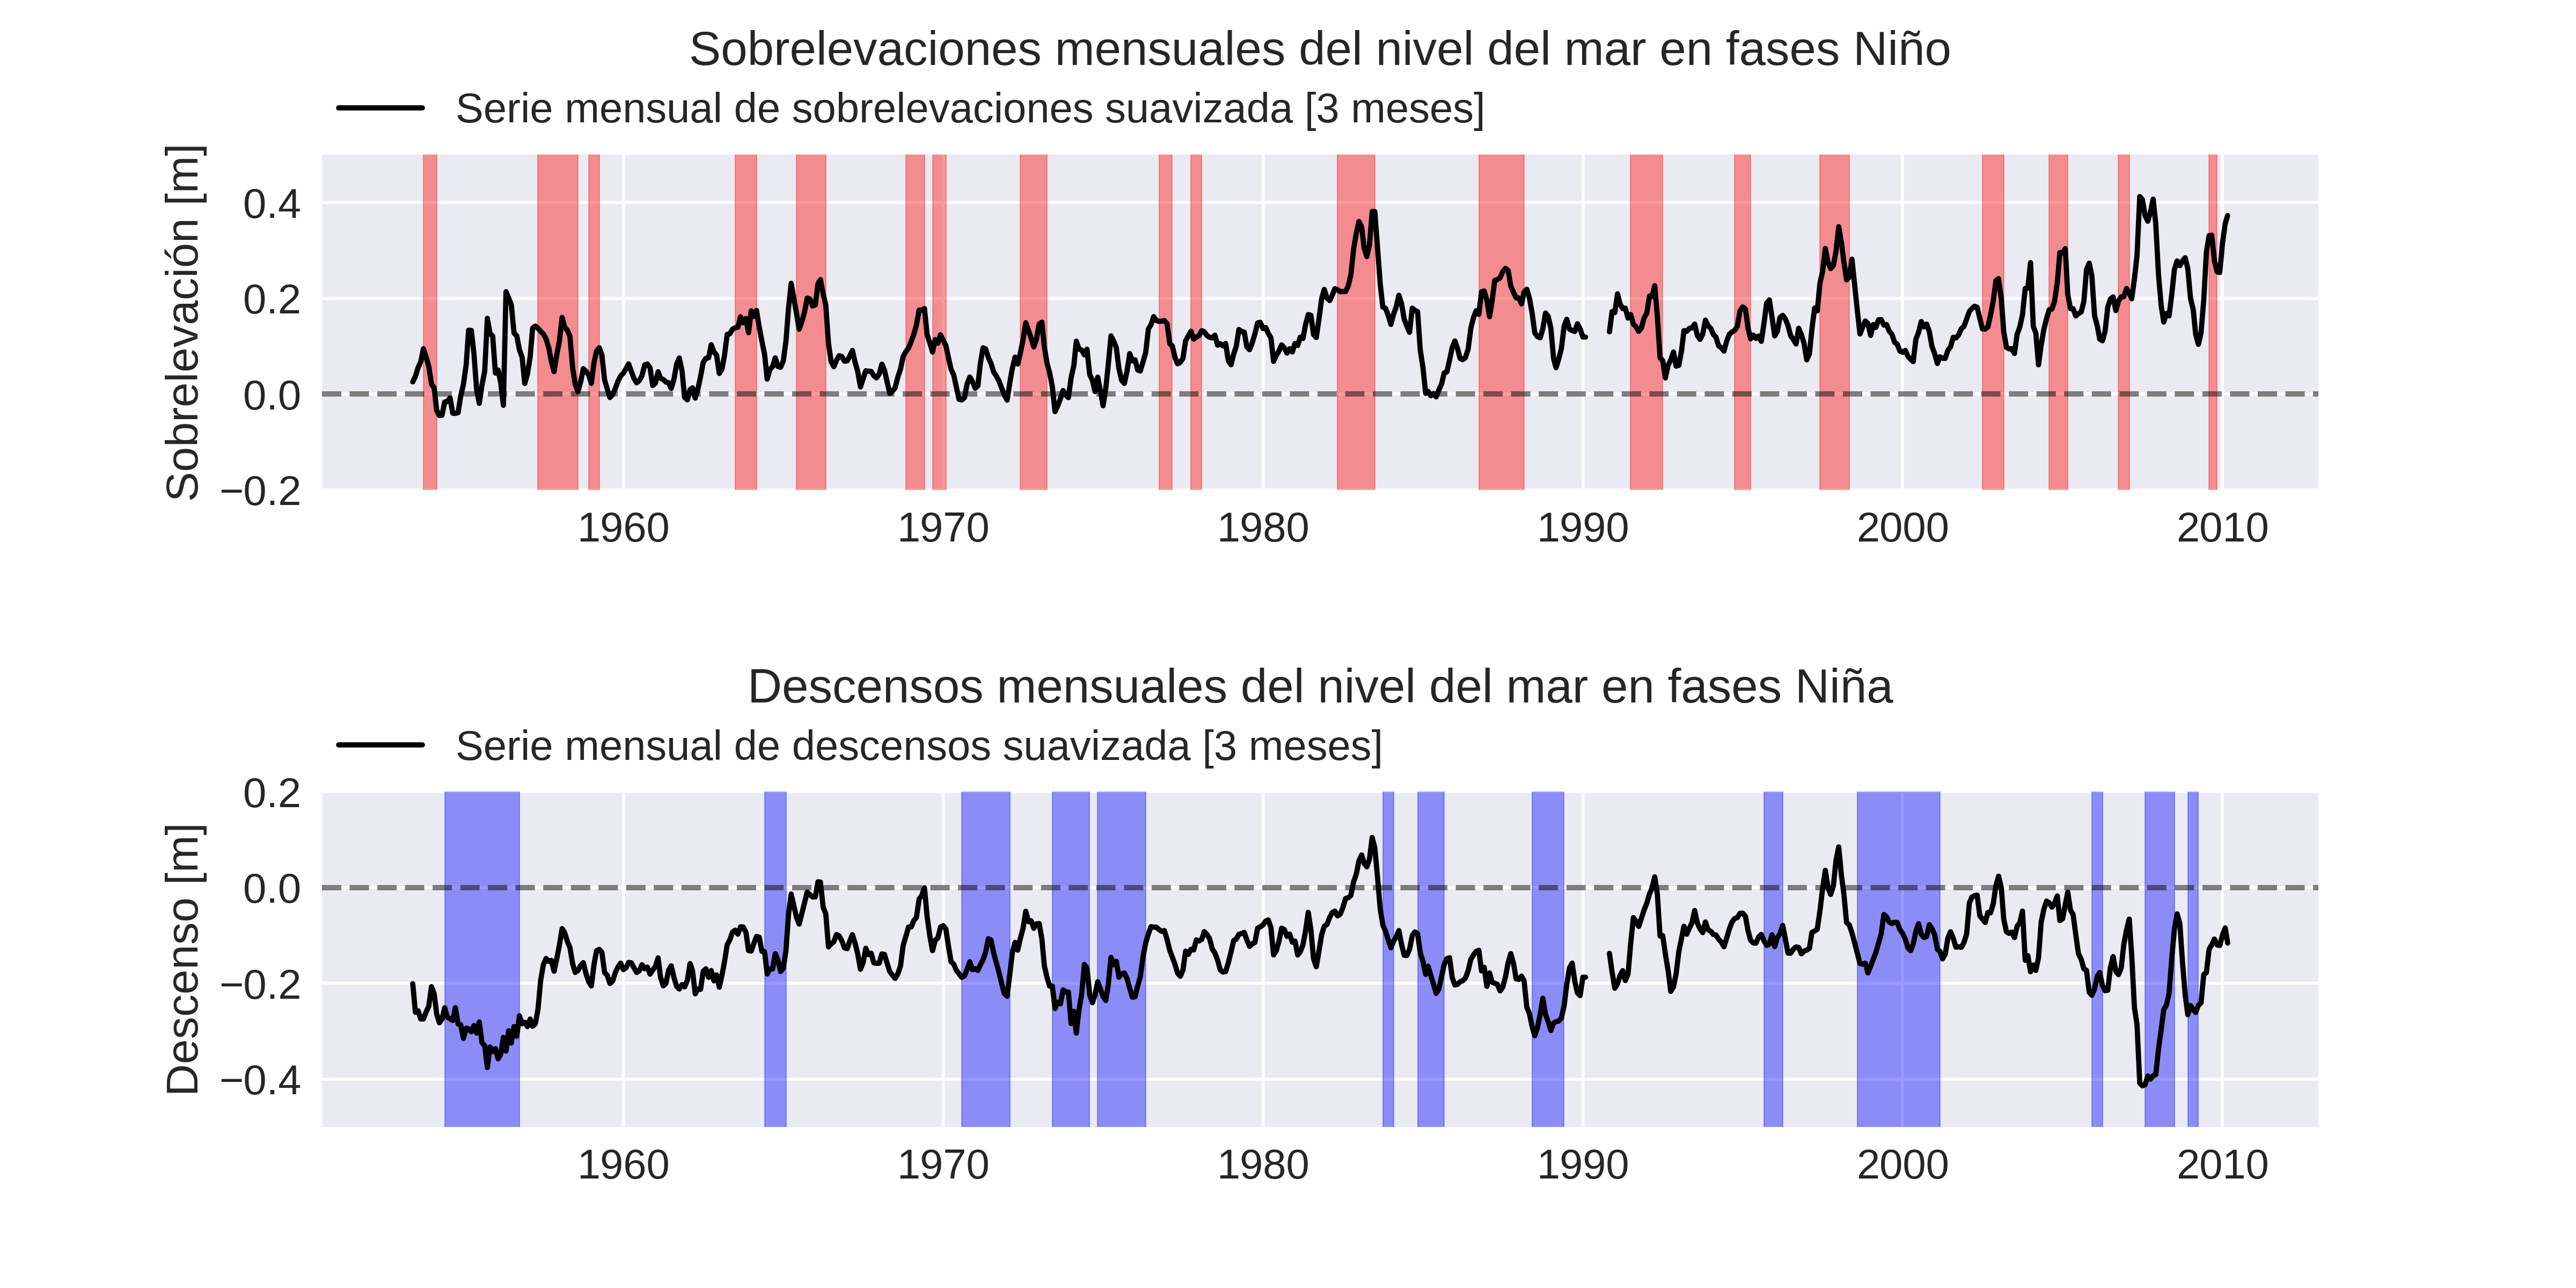
\includegraphics[scale=0.55]{s_d_ENSOS.png}
	\caption{Sobrelevaciones y descensos mensuales del nivel del mar en la bahía de Buenaventura durante diferentes eventos ENSO. Las franjas rojas y azules representan fenómenos Niño y Niña respectivamente.}
	\label{fig:s_d_ENSOS}
\end{figure}

No en todos los meses El Niño/La Niña se presentaron sobrelevaciones o descensos mensuales máximos, dado que es posible que la intensidad de un evento varíe según el estado del océano previo a su inicio.

Adicionalmente, en la figura \ref{fig:sobrelevaciones vs oni} se observa que diferentes aumentos en la serie mensual del nivel mar coinciden temporalmente con aumentos persistentes del índice ONI, es decir, coinciden con la ocurrencia de eventos Niño. De forma paralela, diferentes descensos en la serie mensual coinciden con la ocurrencia de eventos Niña, aunque en menor medida con respecto a los aumentos. Es importante recordar que para que se determine un evento Niño/Niña deben existir valores del índice ONI de +0.5/-0.5 durante tres meses consecutivos.

\begin{figure}[H]
	\centering
	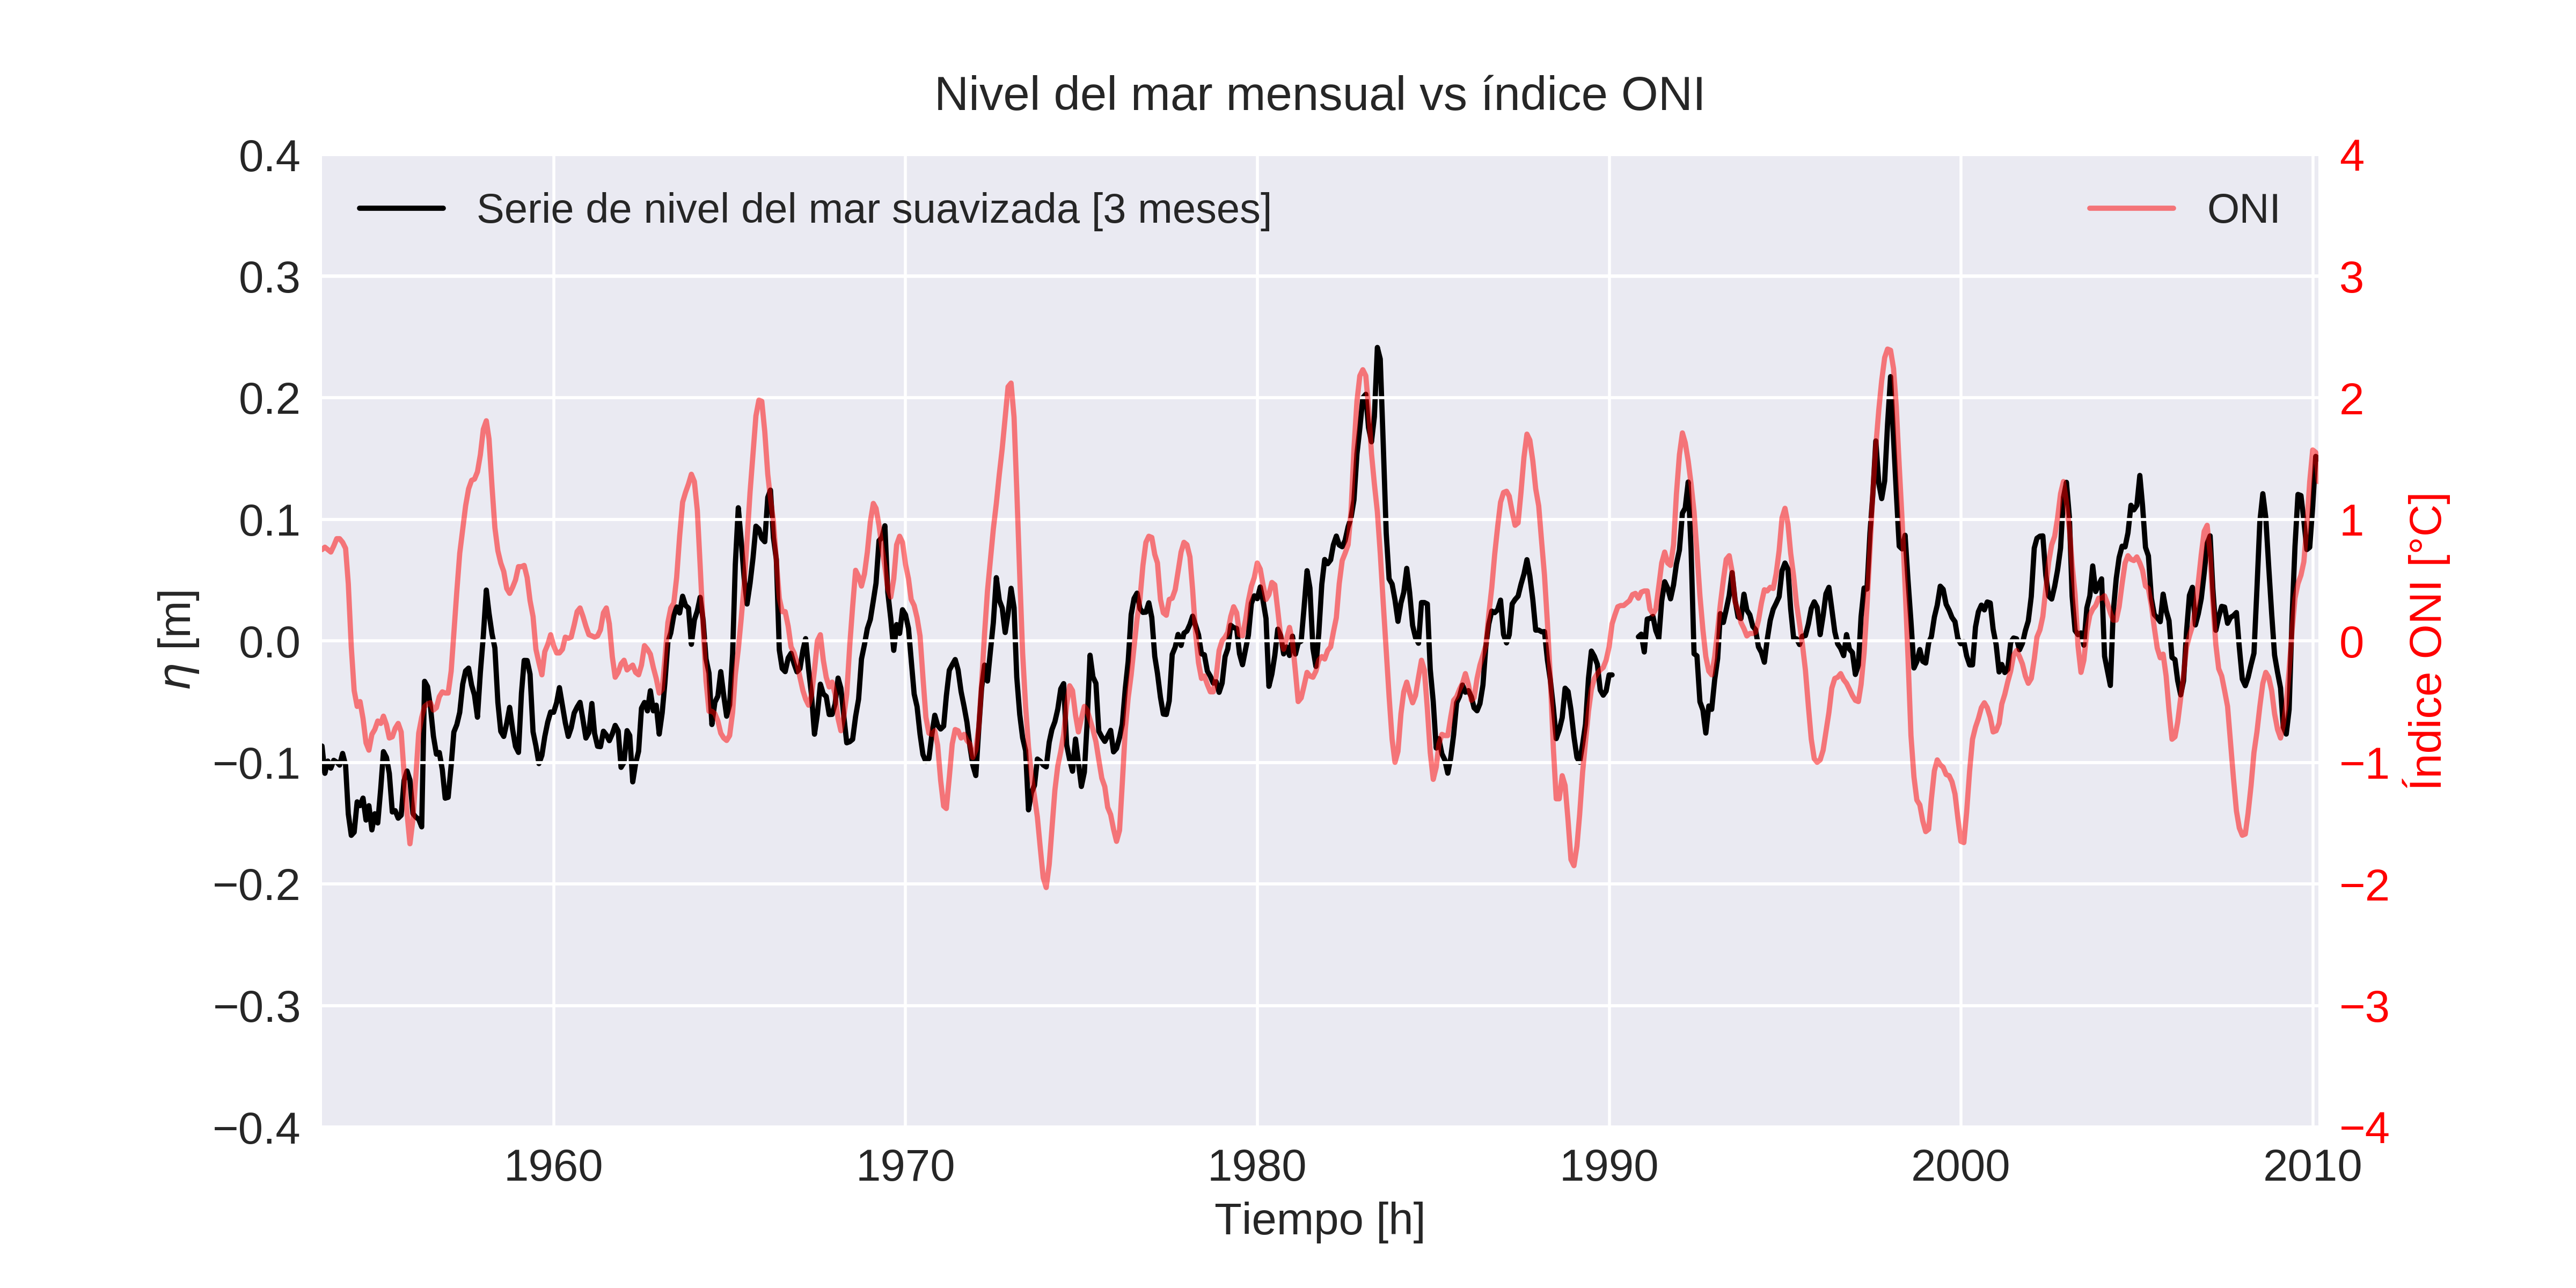
\includegraphics[width=\textwidth]{sobreelev_ONI.png}
	\caption{Sobrelevaciones del nivel del mar en la bahía de Buenaventura vs índice oceánico del niño (ONI) }
	\label{fig:sobrelevaciones vs oni}
\end{figure}

Las figuras \ref{fig:s_d_ENSOS} y \ref{fig:sobrelevaciones vs oni} sugierenn que, en gran medida, existe una relación directa del ENSO con el nivel del mar en la bahía de Buenaventura, aunque sigue siendo necesario caracterizar los eventos Niño y Niña en términos de su duración, sobrelevaciones y descensos máximos así como su comportamiento desde la variable de nivel del mar.

\section{Caracterización de los eventos Niño y Niña}
Desde 1953 hasta 2010 ocurrieron 32 fases cálidas y frías del ENSO, distribuídas en 19 eventos Niño y 13 eventos Niña. De acuerdo a su duración, se clasifican en la siguiente tabla:

\begin{table}[H]
	\centering
	\begin{tabular}{|c|c|c|}
		\hline
		Duración & Cantidad de Eventos Niño&Eventos Niña\\
		\hline
		90 días - 180 días & 7&3\\
		\hline
		180 días - 360 días & 8&4\\
		\hline 
		$>$ 360 días & 4&6\\
		\hline
	\end{tabular}
	\caption{Cantidad de eventos Niño y Niña para cada rango de duración}
	\label{table:eventos_niñ@}
\end{table}

El comportamiento del nivel del mar se ve influenciado durante cada uno de las fases positivas o negativas del ENSO. En la siguiente figura, se presenta cada una de las series de sobrelevacion diaria del nivel asociada a cada una de las fases cálidas del ENSO desde 1953 hasta 2010, también se clasifican según su duración, con la finalidad de captar mejor sus variaciones temporales. La serie de sobrelevaciones diarias se promedia en ventanas móviles de 2 meses con el fin de obtener sólo variaciones temporales desde la escala trimestral.

\begin{figure}[H]
	\centering
	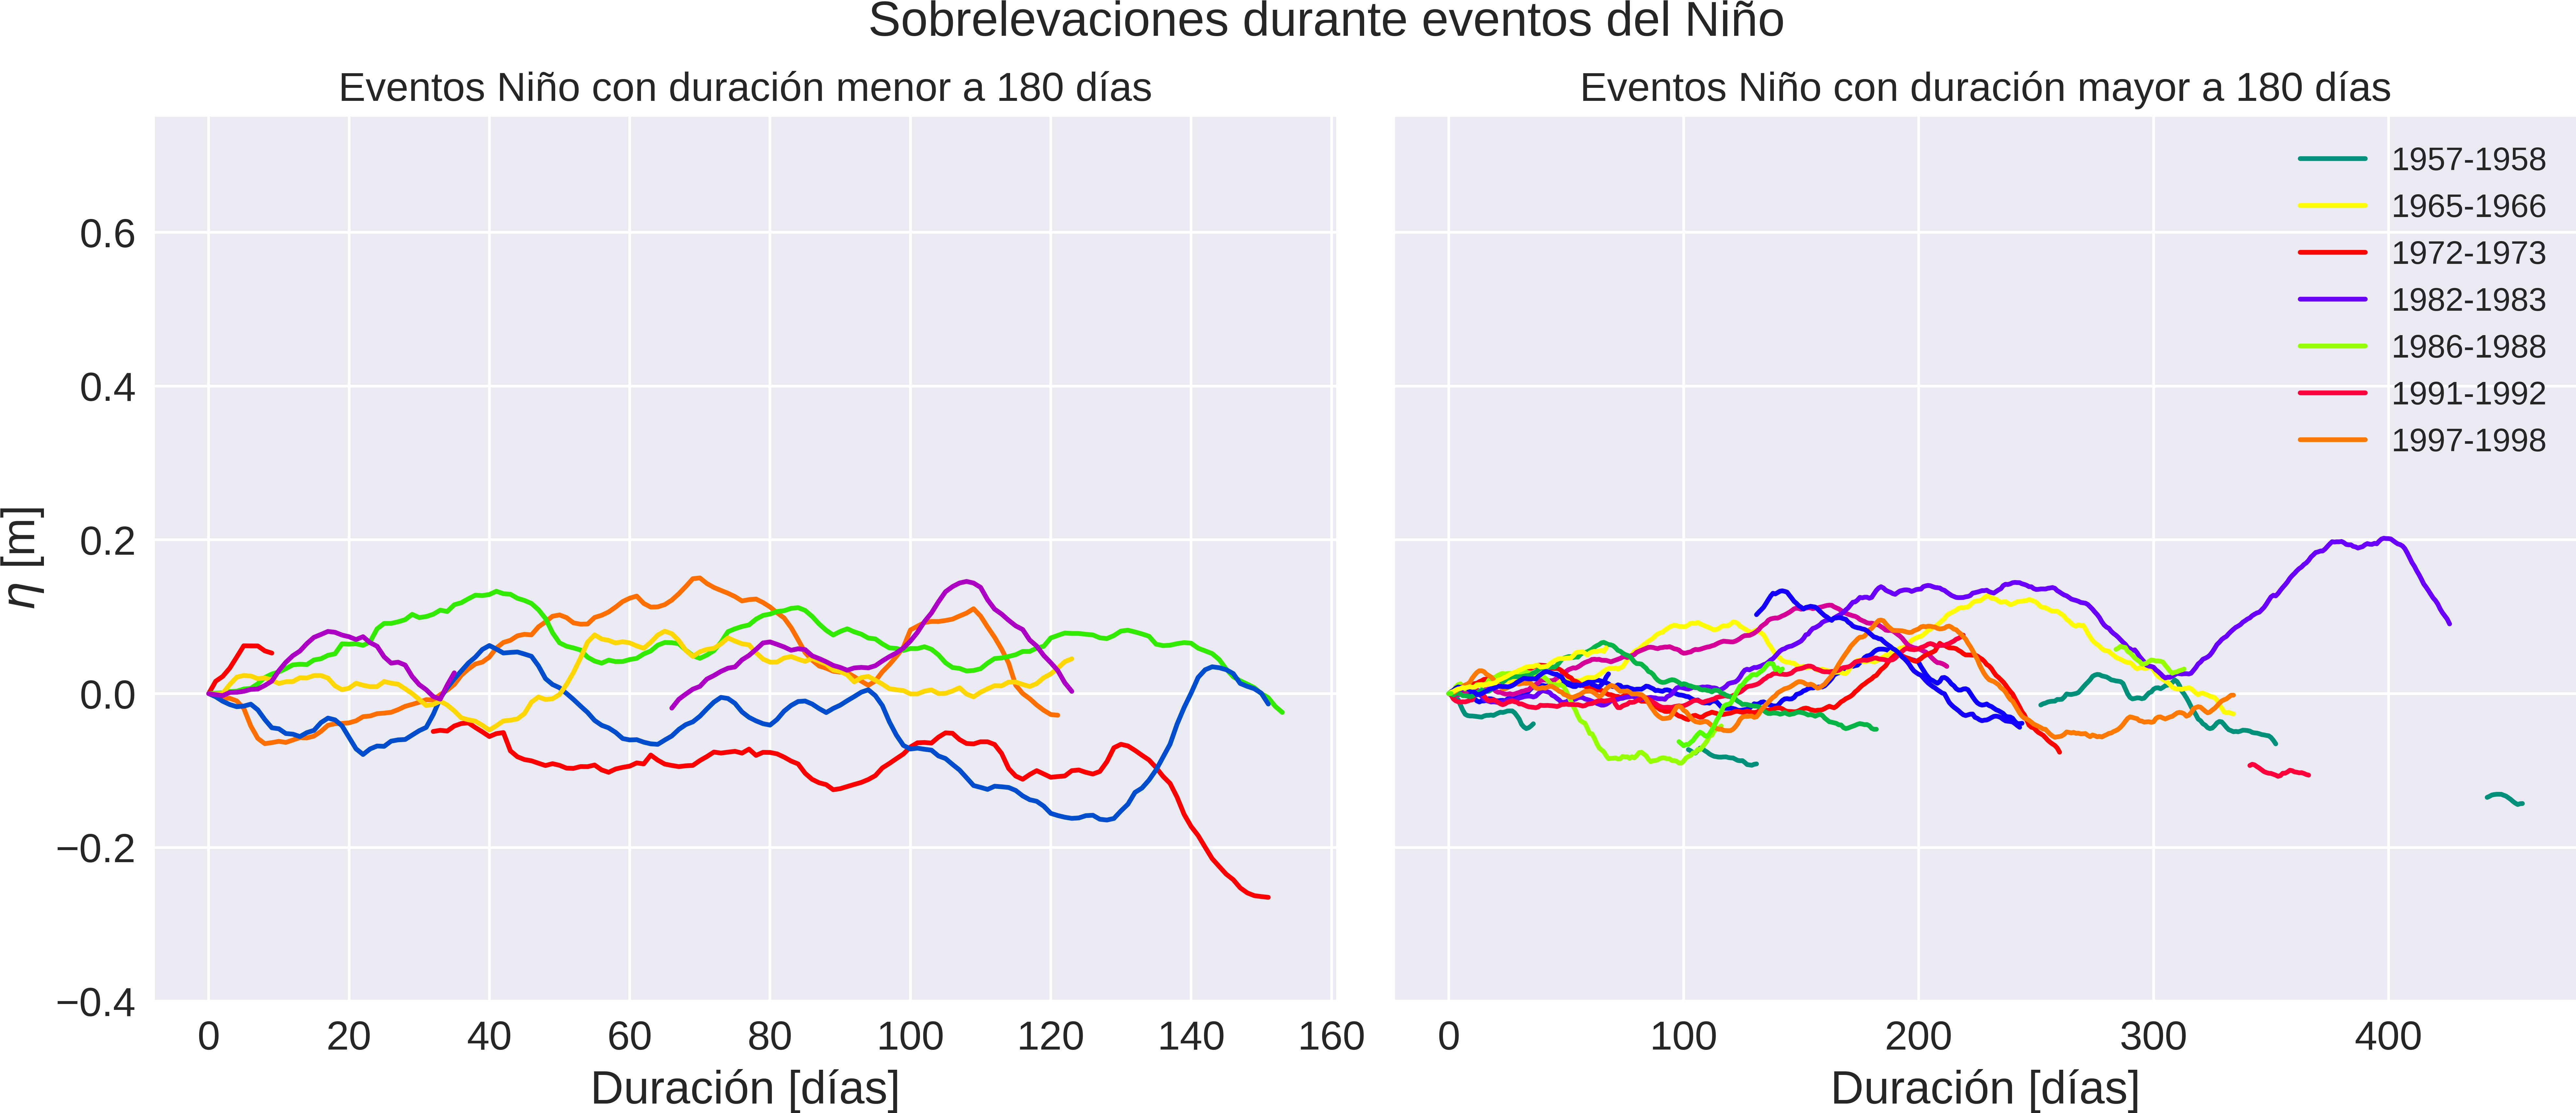
\includegraphics[width=\textwidth]{nino_events.png}
	\caption{Sobrelevaciones del nivel del mar Bajo diferentes duraciones de eventos ENSO}
	\label{fig:nino_events}
\end{figure}

\begin{itemize}
	\item Eventos con duración entre 90 días-180 días: En este rango de duración es en el único dónde el nivel del mar se mantuvo constante para algunos eventos Niño, esto puede asociarse a que estos eventos fueron menos intensos y menos estables que otros de mayor duración. Además, tendencias negativas durante ciertas fases cálidas sugieren la coexistencia de otros fenómenos que no favorecen el descenso del nivel.
	
	\item Eventos con duración entre 180 días-360 días: Durante estos eventos, el comportamiento de nivel del mar se parece más al esperado, puesto mientras se desarrolla el evento se presentan momentos de crecimiento y decrecimiento del nivel, inclusive empiezan a aparecer ciertos períodos de 3 meses, que podrían asociarse con las ondas Kelvin que traviesan el pacífico ecuatorial desde Oeste a Este y logran arribar a las costas suramericanas debido al debilitamiento de los vientos alisios del Este. La mayoría de los eventos Niño se concentraron entre estas duraciones.
	
	\item Eventos con duración mayor a 360 días: El nivel del mar durante los eventos que duraron más de un año tiene características similares a los anteriores, con períodos de 3 meses marcados y con períodos más largos cercanos a los 6 meses.
	
\end{itemize}

Un resumen general tanto de la duración como de las sobrelevaciones máximas que generaron estos eventos se observa a continuación:

\begin{figure}[h]
	\centering
	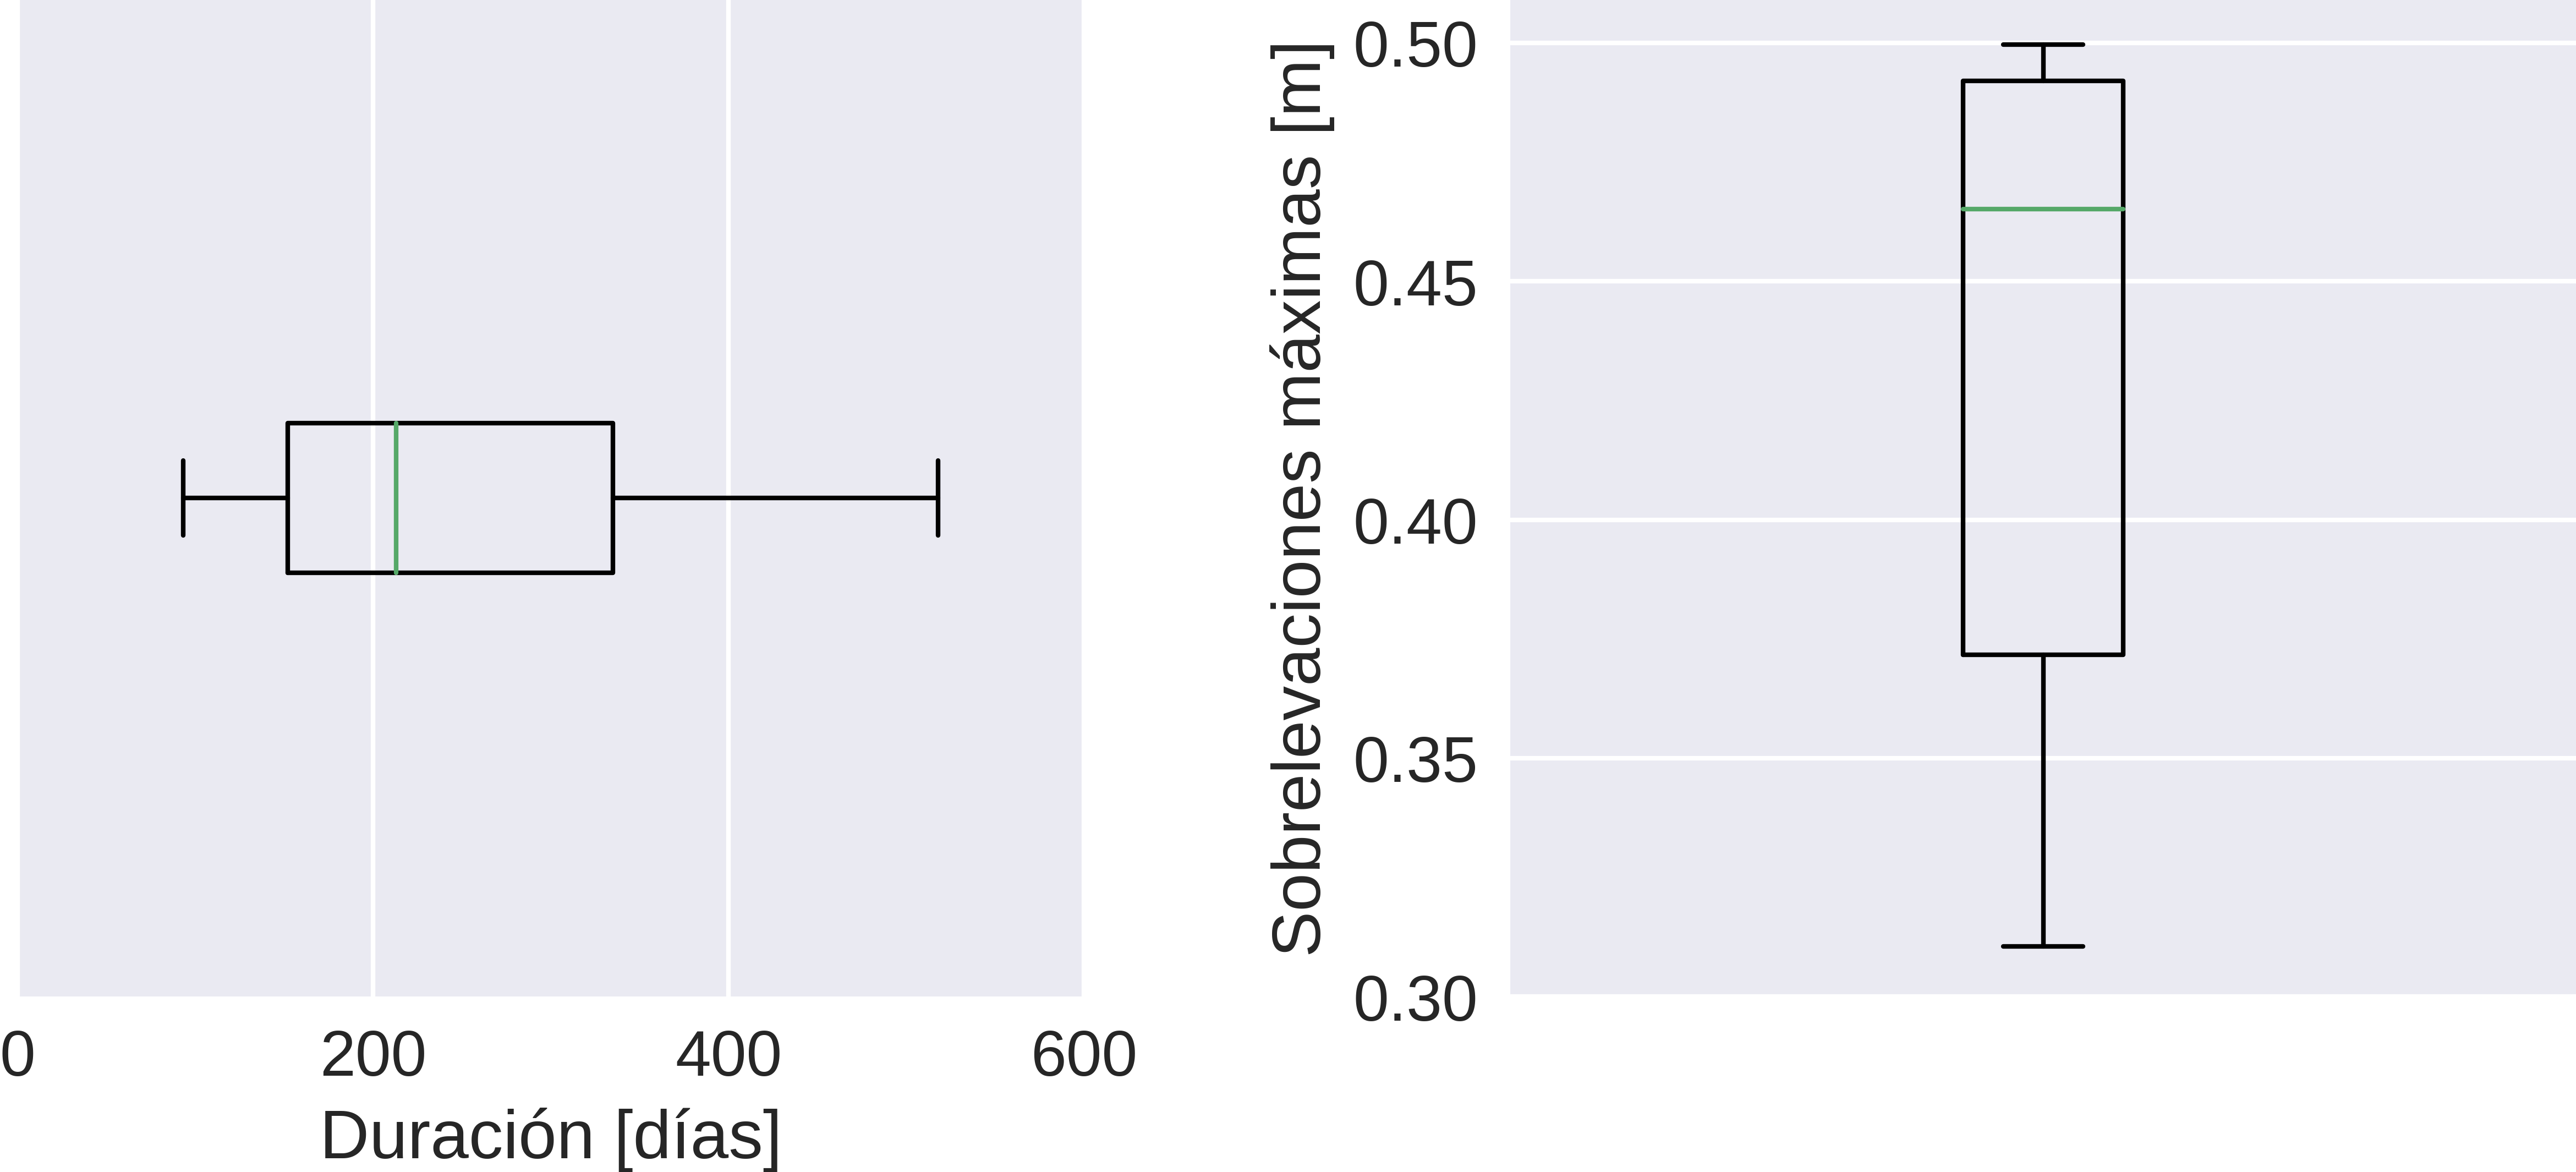
\includegraphics[scale=0.7]{durs_nino_events.png}
	\caption{Diagramas de caja y bigotes para las duraciones y sobrelevaciones máximas durante los eventos Niño desde 1953 hasta 2010}
	\label{fig:durs_nino}
\end{figure}

La duración promedio de los eventos Niño que ocurrieron entre 1953 y 2010 fue de 260 días, aunque se resalta que el 75\% de estos eventos duraron menos de 335 días. El evento que más duró fue el Niño 1986-1987 (518 días). La menor sobrelevación que se generó durante estos eventos fue de 31.0 cm, y se generaron sobrelevaciones promedio de 43.3 cm y la mayor se originó mientras transcurría el evento Niño 1982-1983, se recuerda especialmente la sobrelevación durante 1997-1998, justo en el período dónde un comunidad costera de la bahía de Buenaventura llamada Punta Soldado se vio obligada a reubicarse por al aumento súbito del nivel del mar \footnote{En el archivo digital de noticias el tiempo aparece el reporte \url{https://www.eltiempo.com/archivo/documento/MAM-273680}}
%
Para el estudio de los eventos Niña también se grafican las series de descensos diarios promediadas en ventanas móviles de 2 meses y se clasifican según su duración (Fig. \ref{fig:nina_events}).

\begin{figure}[H]
	\centering
	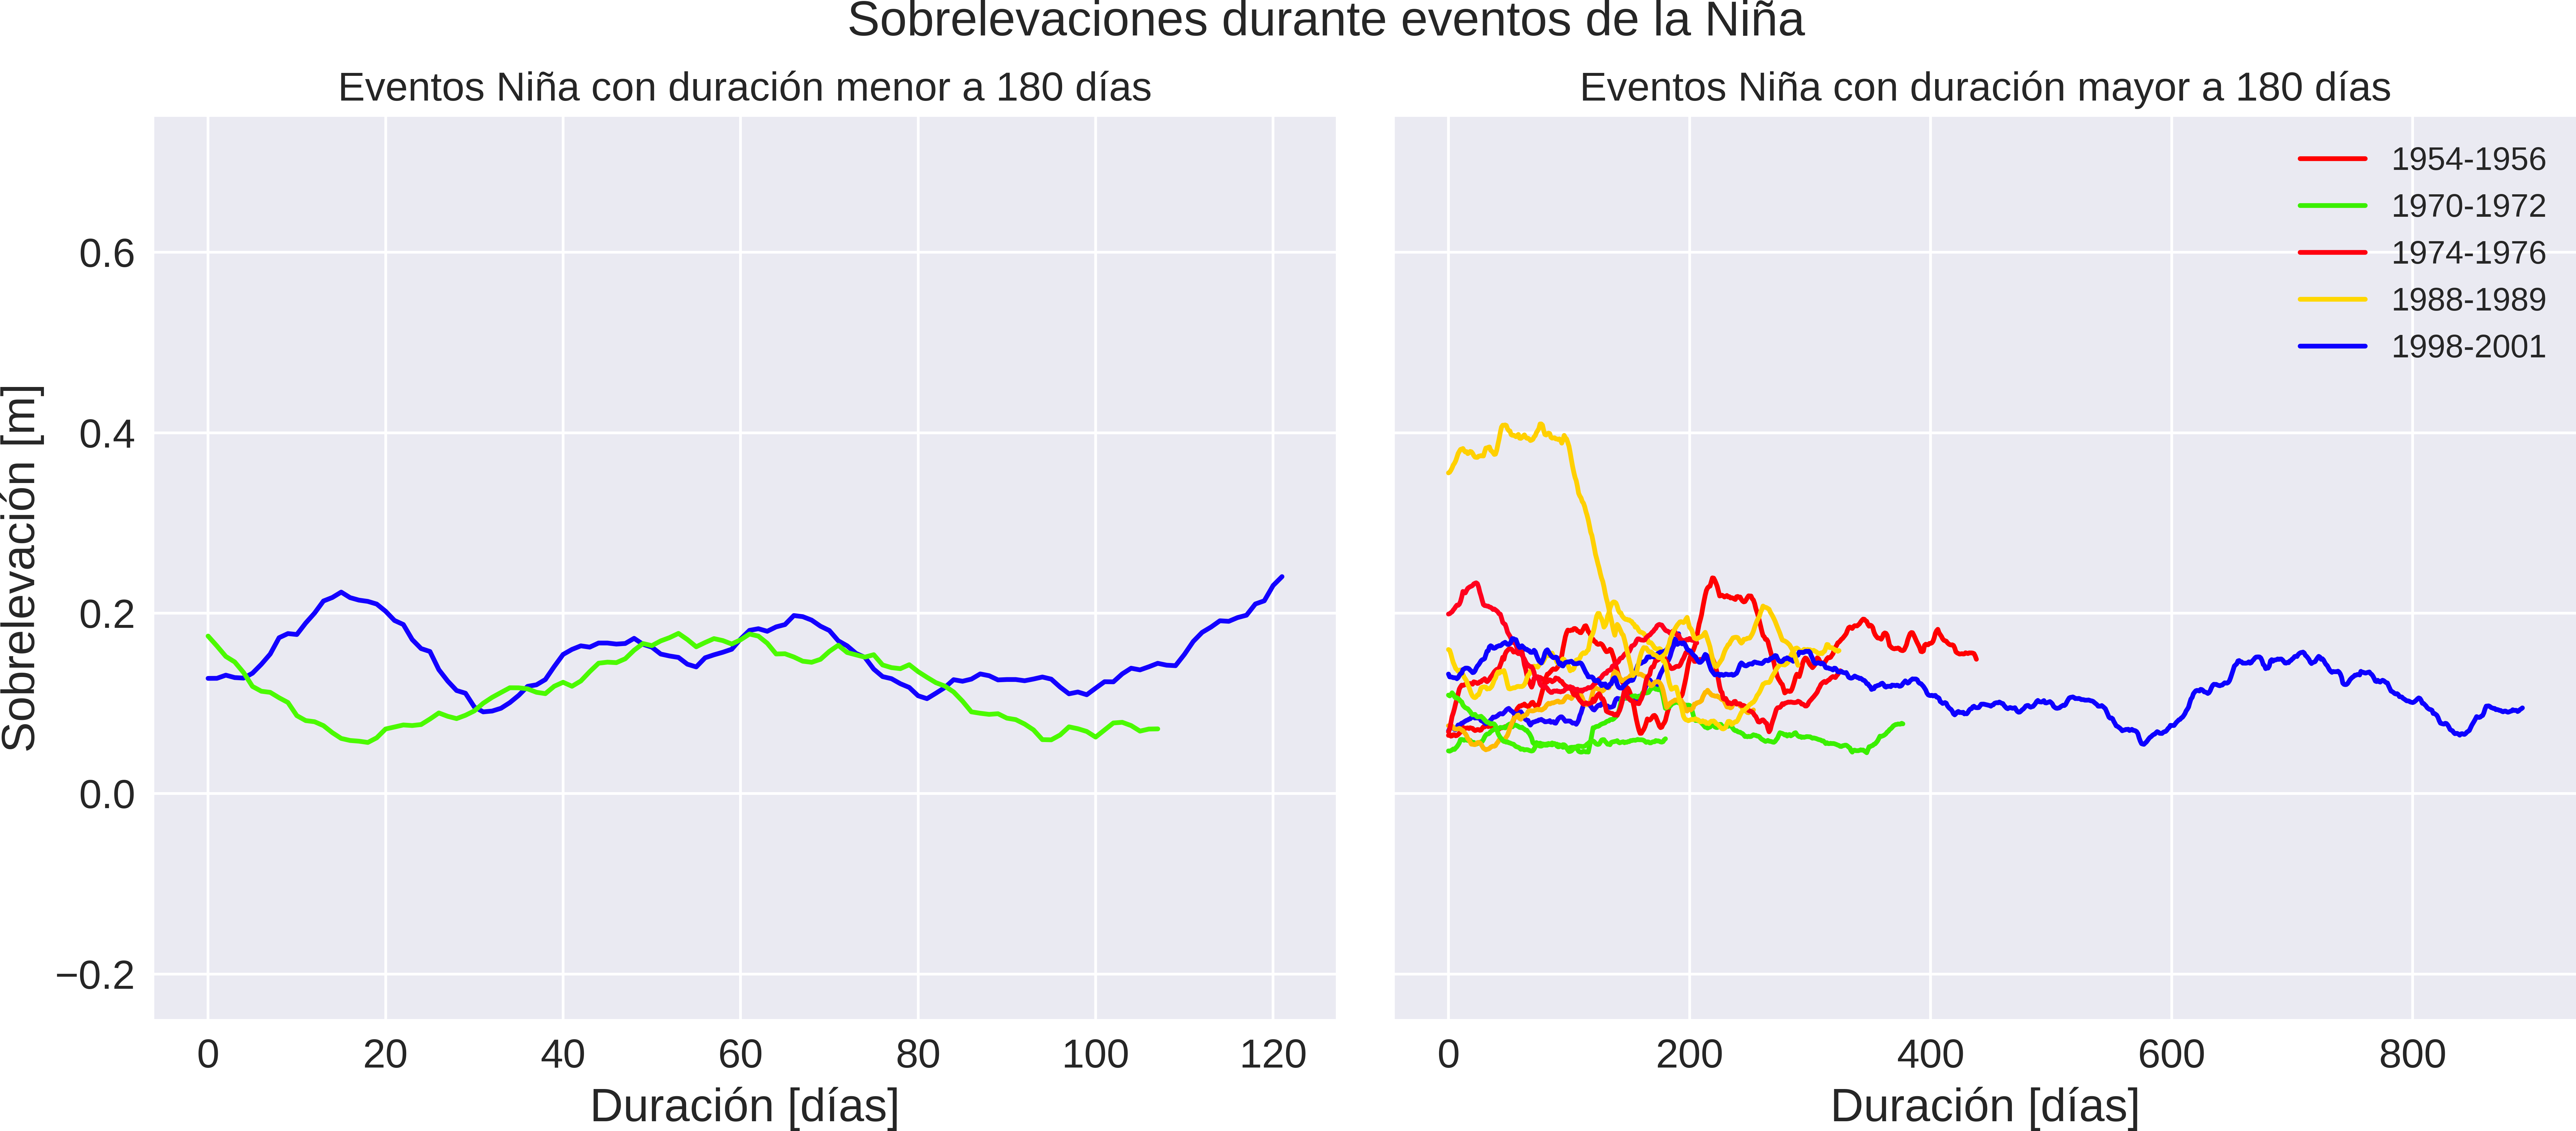
\includegraphics[width=\textwidth]{nina_events.png}
	\caption{Descensos del nivel del mar bajo diferentes duraciones de eventos Niña}
	\label{fig:nina_events}
\end{figure}

\begin{itemize}
	\item Eventos con duración entre 90 días-180 días: Sólo 3 eventos Niña están enmarcados entre estas duraciones, e incluso durante algunos se presentaron sobrelevaciones del nivel. Esto parece indicar que deben existir ciertas condiciones adicionales para que se genere un descenso del nivel del mar mientras ocurre un evento Niña. 
	
	\item Eventos con duración entre 180 días-360 días: El comportamiento del nivel durante estos eventos es más similar entre sí, con descensos más pronunciados (-5 cm a -20 cm) y con variaciones períodicas cercanas a los 3 meses y que podrían deberse a las respuestas oceánicas de las ondas Kelvin, llamadas ondas Rossby. Se resalta un evento durante el cuál, el nivel descendió hasta -40 cm al inicio y empezó a aumentar hasta llegar al nivel medio aproximadamente, es decir, no tuvo variaciones períodicas.
	
	\item Eventos con duración mayor a 360 días: La mayoría de los eventos se concentran en estas duraciones (6 de los 13 ocurridos). Durante ciertos fenómenos de mayor duración, el nivel del mar, aunque desciende, se mantiene dentro de ciertos valores; para otros fenómenos el nivel del mar desciende periódicamente. Los eventos Niña más largos en esta categoría superan en duración a los eventos Niño más largos presentados desde 1953 a 2010. 
	
\end{itemize}

Los diagramas de la figura \ref{fig:durs_nina} explican la distribución de las duraciones y de los descensos máximos ocurridos durante eventos Niña:

\begin{figure}[h]
	\centering
	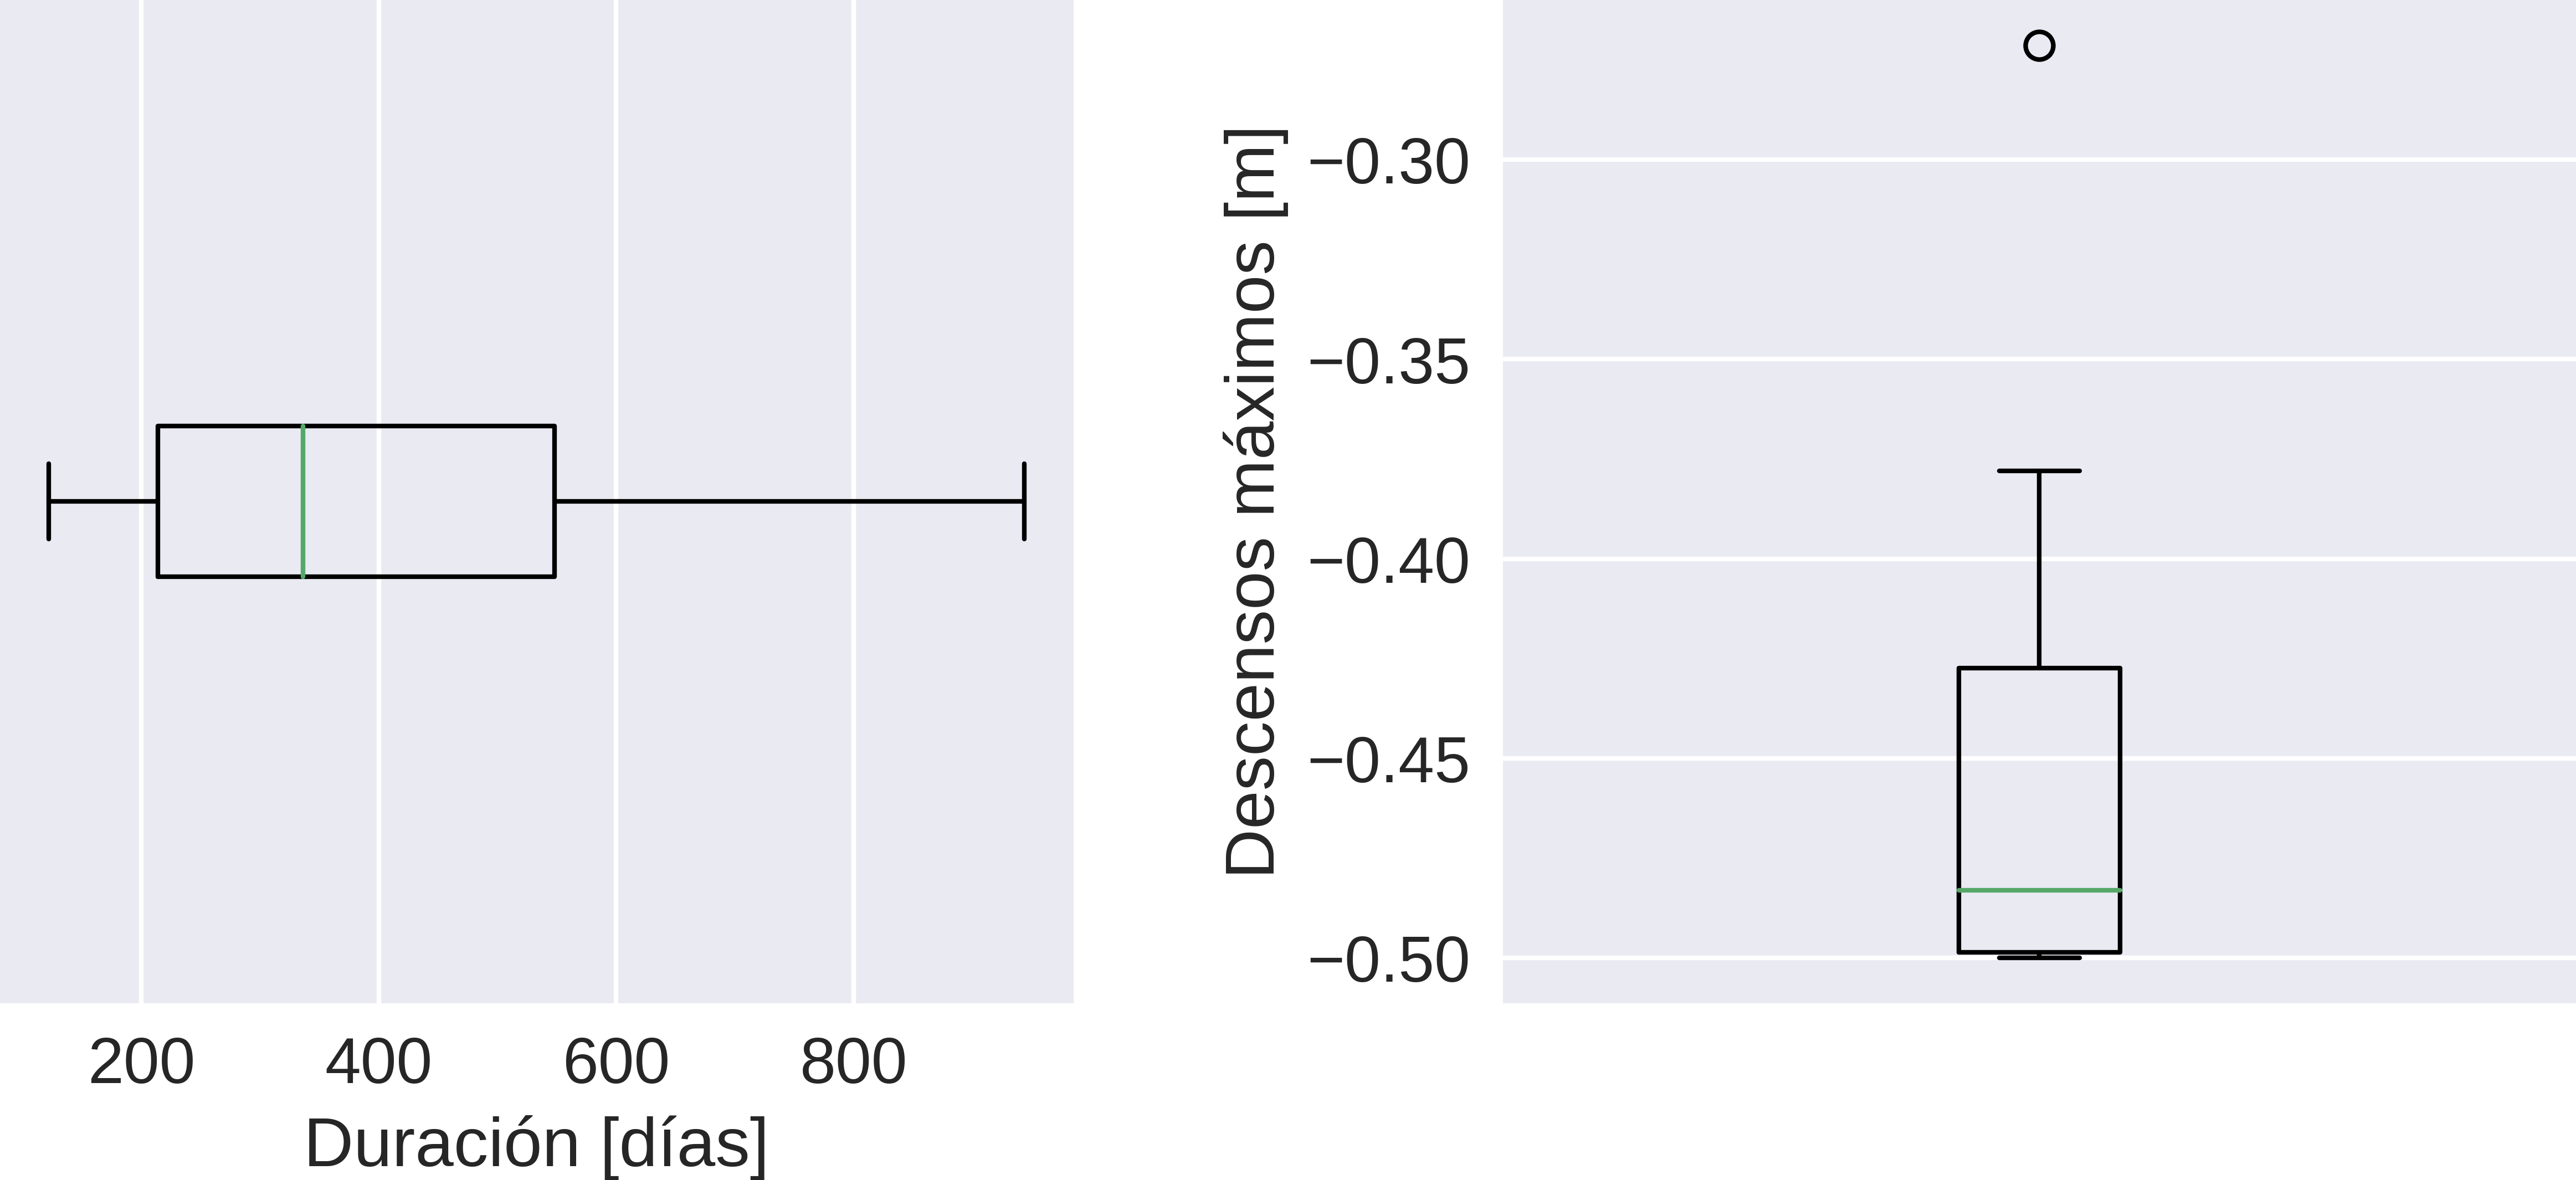
\includegraphics[scale=0.7]{durs_nina_events.png}
	\caption{Diagramas de caja y bigotes para las duraciones y sobrelevaciones máximas durante los eventos Niña desde 1953 hasta 2010}
	\label{fig:durs_nina}
\end{figure}

La duración promedio de los eventos Niña que ocurrieron entre 1953 y 2010 fue de 397 días, aunque se resalta que el 75\% de estos eventos duraron menos de 335 días. El evento que más duro fue la Niña 1998-2001 (944 días). El mayor descenso que se generó durante estos eventos fue de 49.9 m, y el descenso promedio es cercano a los 45.2 m.

Se resalta que la máximas sobrelevaciones o descensos del nivel del mar no siempre se generaron en la mitad de la duración de cada evento, inclusive en algunos eventos no se generaron sino hasta el final. Esto genera una pregunta acerca de cómo otras condiciones condiciones locales presentes, tales cómo los vientos, el efecto de la bahía, la época del año, entre otros, pueden modular el nivel del mar durante estos eventos Niño o Niña

De las figuras \ref{fig:nino_events} y \ref{fig:nina_events} se puede notar que durante muchos de los fenómenos del Niño y de la Niña, el nivel del mar alcanza aumentos y descensos máximos prolongados que amenazan las condiciones en las comunidades costeras. Ahora bien, es importante resaltar que, el hecho de que haya sobrelevaciones máximas y descensos máximos durante eventos Niño y Niña, no implica que toda la amplitud de la sobrelevación o descenso se deba al ENSO. Surge entonces la necesidad de caracterizar los aportes al nivel del mar por parte de este fenómeno y para ello debe realizarse un análisis espectral.
%
\section{Análisis espectral}

Dado que el nivel del mar varía en diferentes escalas de tiempo y se deben identificar las componentes más importantes en el dominio de las frecuencias, se realizó el análisis espectral a la serie mensual de nivel del mar del mareógrafo

\begin{figure}[h]
	\centering
	\includegraphics[scale=0.5]{Fourier.png}
	\caption{El espectro de potencias de Fourier en el lado izquierdo de la figuro y la banda espectral de interés en el lado derecho}
	\label{fig:fourier}
\end{figure}

En el lado izquierdo de la figura \ref{fig:fourier} se muestra el espectro de potencias de Fourier, en el se puede notar que hay períodos dónde hay mayor concentración de la energía, uno de estos es alrededor de 6 meses asociado al ciclo semianual, otros valores donde hay concentración de la energía están en períodos superiores a los 12 meses. El ENSO, al ser un fenómeno que sucede en la escala interanual, es suficiente que se estudie entre períodos de 2 y 6 años, por lo tanto, las demás potencias asociadas a otras escalas temporales no se tomaron en cuenta, como lo indica el lado derecho de la figura \ref{fig:fourier}. La varianza en esta banda de interés explica el 23.3\% de la varianza total de la serie de nivel del mar.

Se filtra la serie de nivel del mar en la banda espectral de interés con ayuda de la transformada de Fourier inversa. 

\begin{figure}[H]
	\centering
	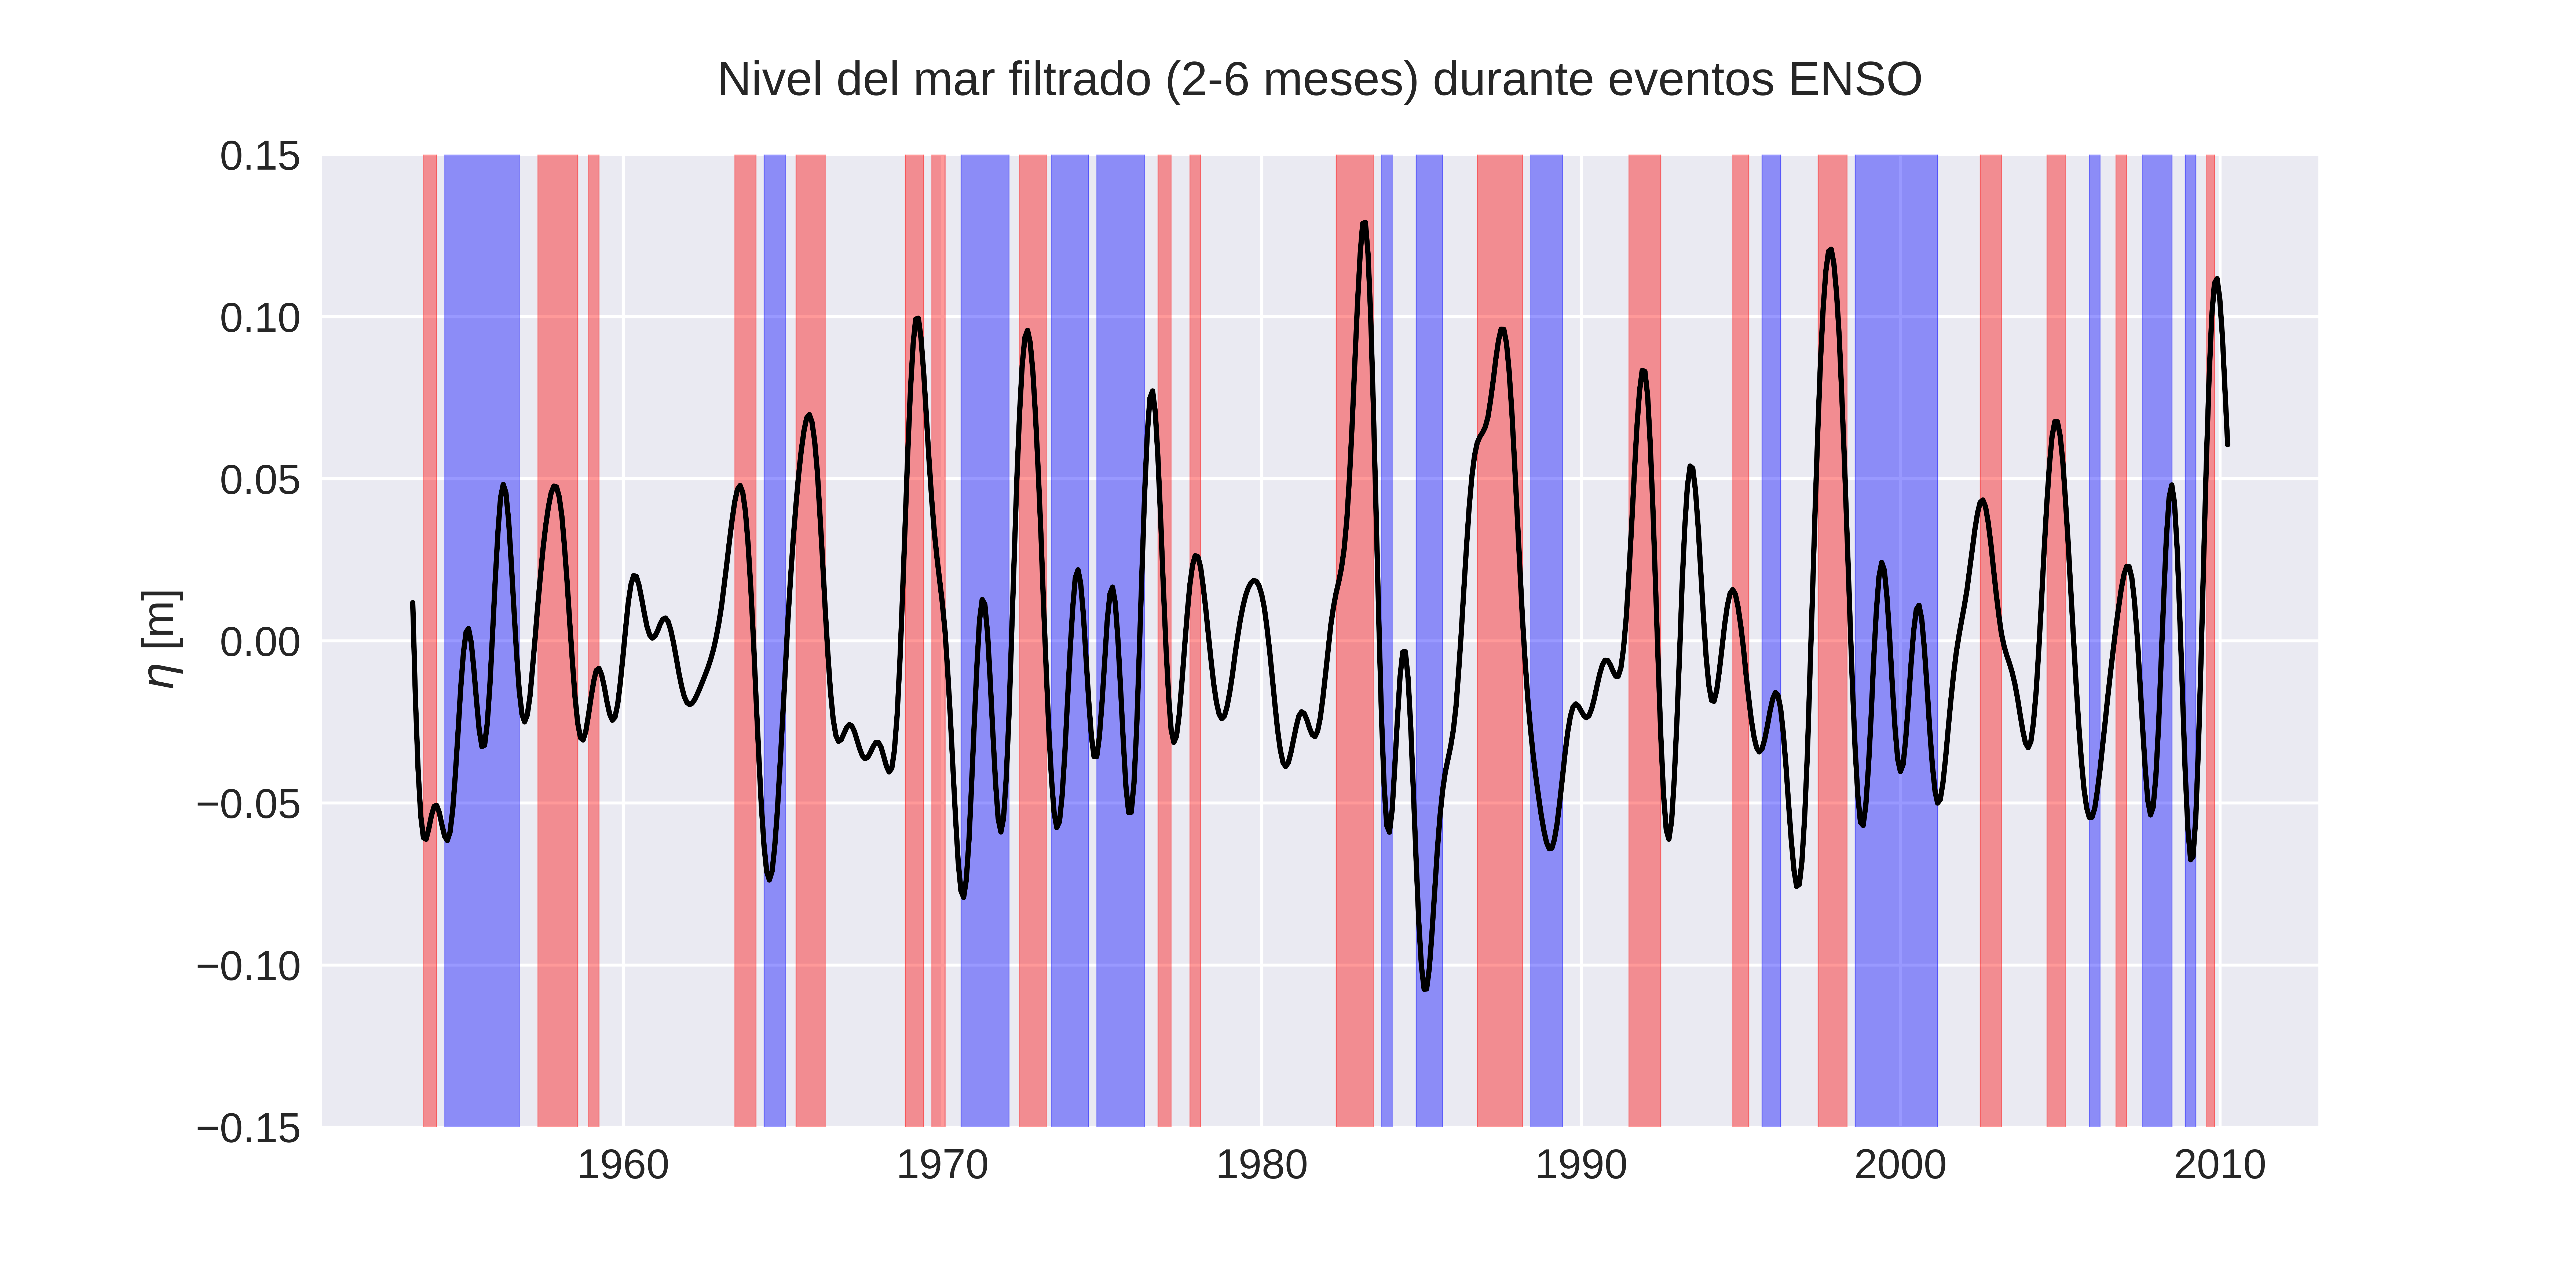
\includegraphics[scale=0.5]{Fourier_Inverso.png}
	\caption{Serie de nivel del mar sólo con la variabilidad comprendida entre 2-6 años}
	\label{fig:fourier_inverso}
\end{figure}

En la figura \ref{fig:fourier_inverso} se evidencia que el nivel del mar enmarcado en la variabilidad interanual, incrementó durante las fases cálidas del ENSO y disminuyó durante las fases frías, lo anterior se comprendió mejor cuando esta serie se comparó con la serie del índice ONI (\ref{fig:fourier vs oni}) y se observaron sobrelevaciones de hasta 10 cm que coinciden con fases cálidas.

\begin{figure}[H]
	\centering
	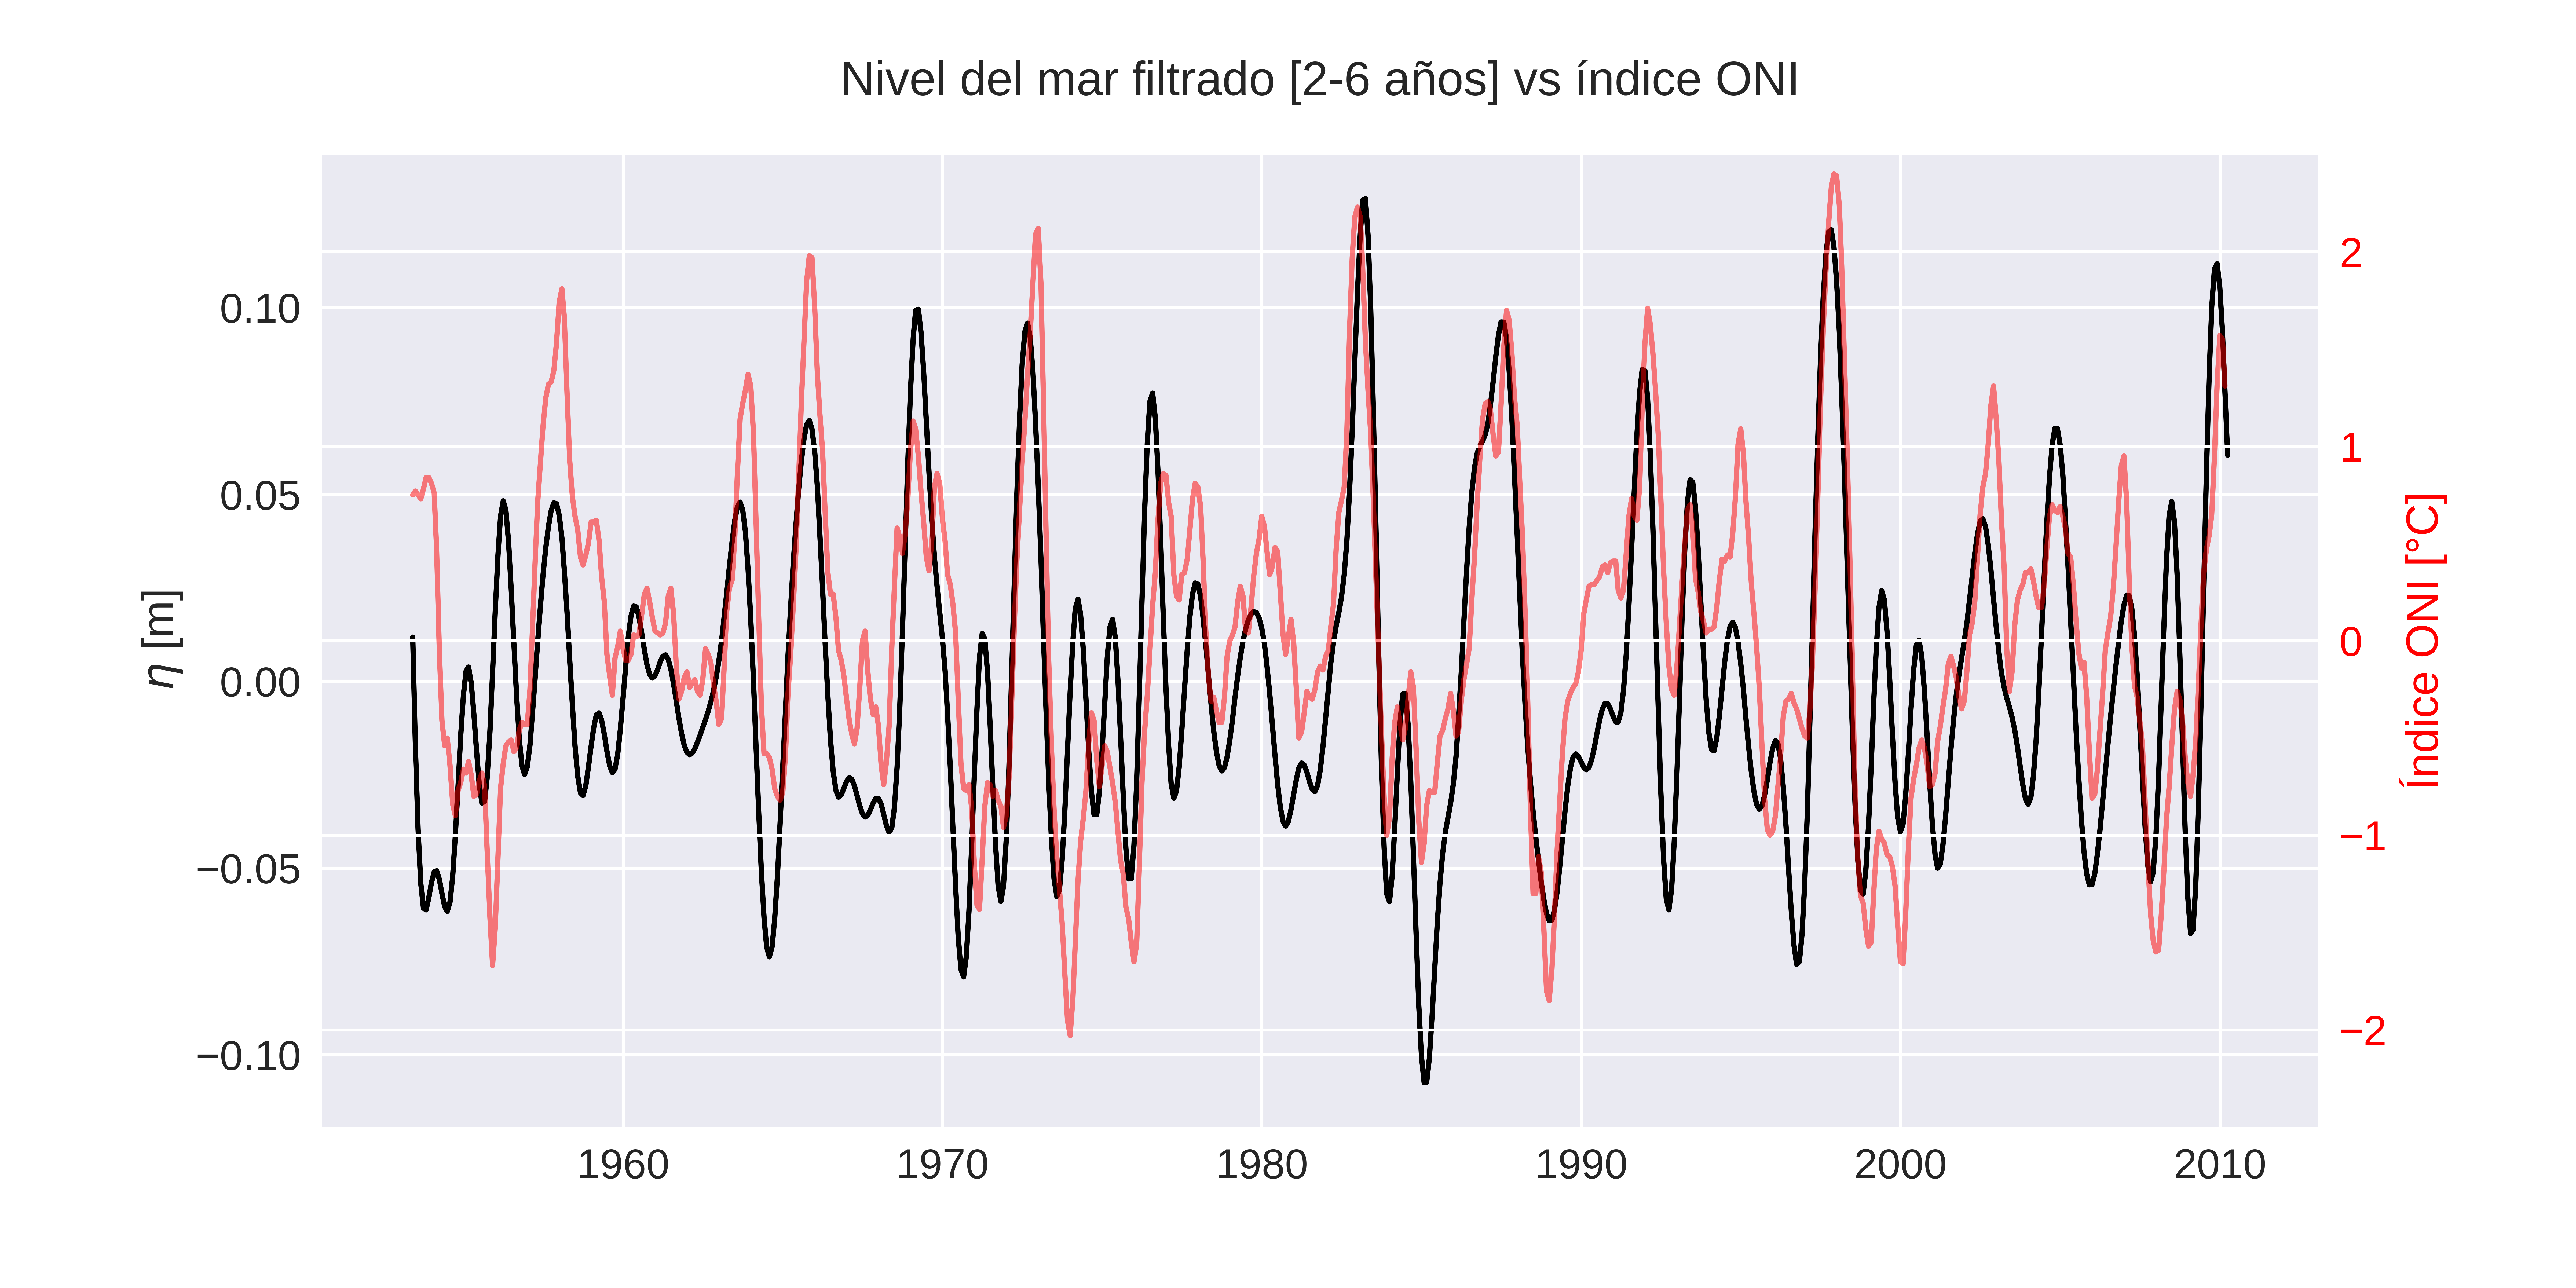
\includegraphics[scale=0.5]{Fourier_ONI.png}
	\caption{Serie de nivel del mar sólo con la variabilidad comprendida entre 2-6 años}
	\label{fig:fourier vs oni}
\end{figure}


\section{Variabilidad espacial del nivel del mar en el Pacífico Tropical}

Conocidas las sobrelevaciones y descensos del nivel del mar que se pueden generar en una región como la bahía de Buenaventura, es fundamental investigar sí dichas perturbaciones del nivel ocurrieron previamente en otras regiones del Pacífico tropical o sí hay variables que se correlacionan con él en determinadas regiones. Esto implica estudiar la variabilidad espacial del nivel del mar y el efecto del ENSO sobre ella.

El primer resultado en este enfoque es el porcentaje de varianza que representa la banda espectral en la que se estudia el ENSO (Fig. \ref{fig:fourier}) en relación a la varianza total del nivel del mar. Lo anterior ayuda estimar cuánto podría influir el ENSO en la variabilidad temporal de esta variable en toda la región del Pacífico tropical.

\begin{figure}[t]
	\centering
	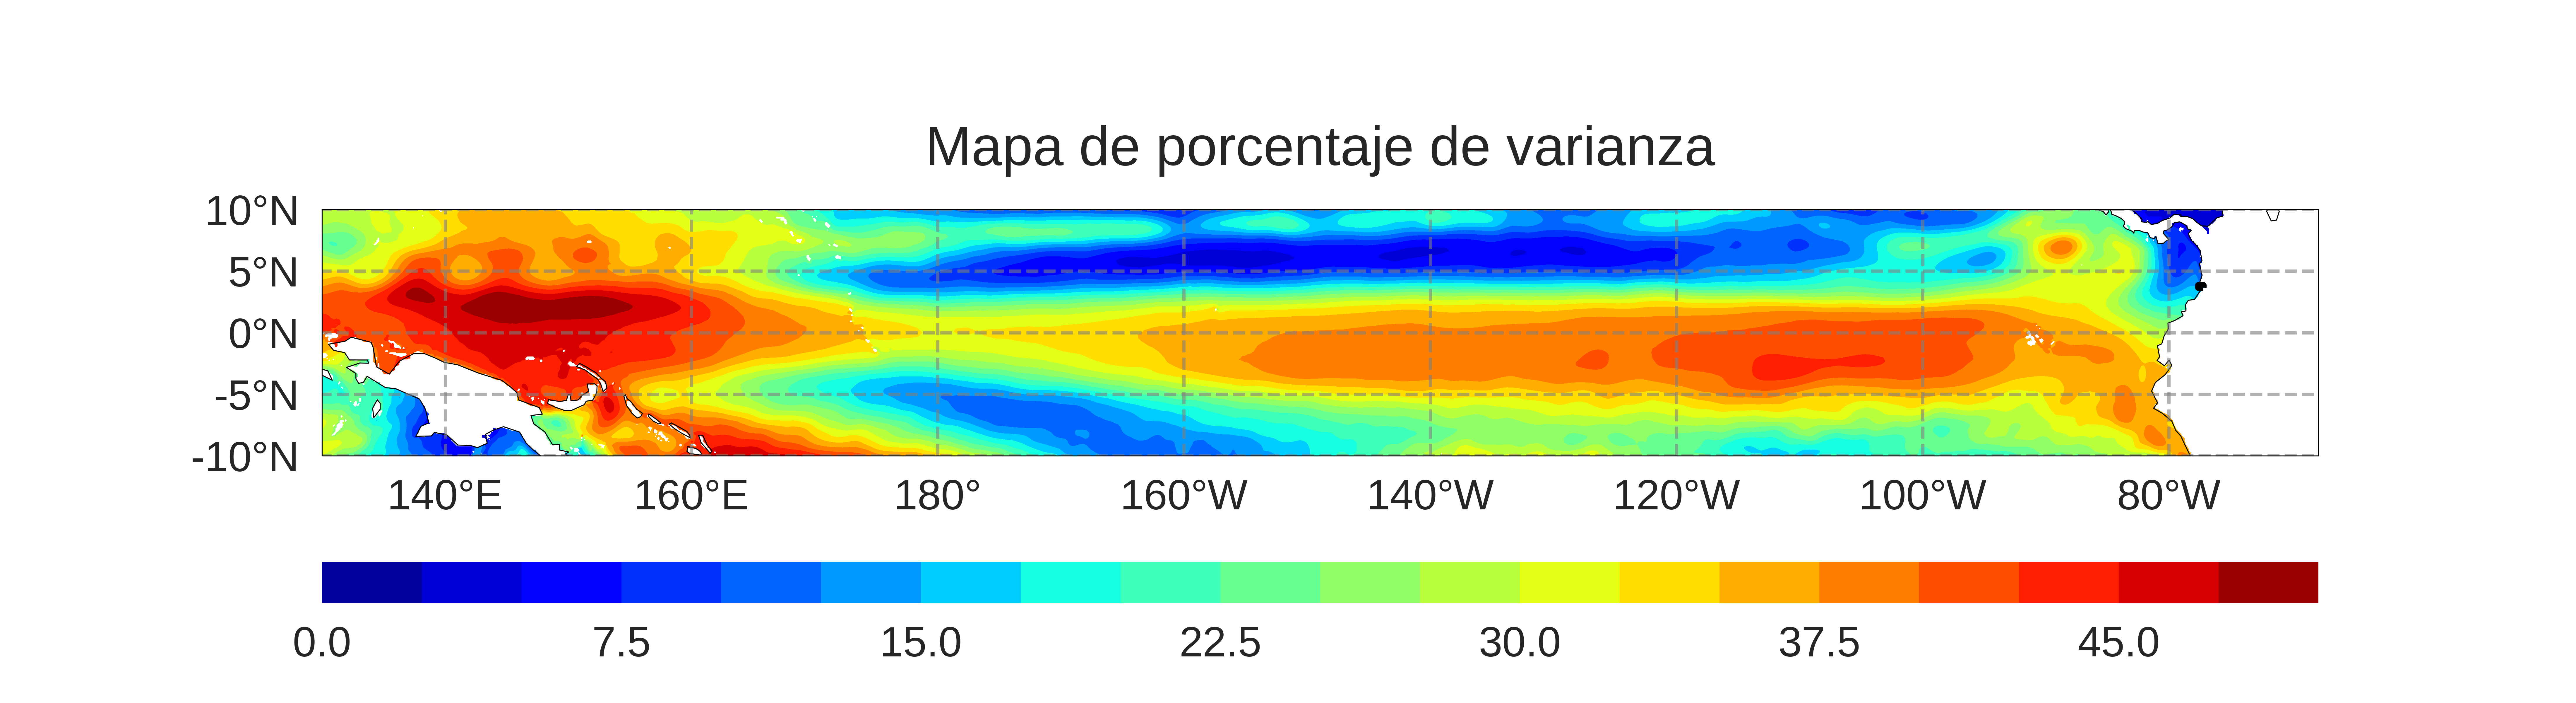
\includegraphics[width=1.1\textwidth]{Mapa_porcentaje_varianza.png}
	\caption{Mapa de porcentaje de varianza}
	\label{fig:porcentaje_varianza}
\end{figure}

En diferentes zonas como las piscina caliente y la región que abarca la lengua fría del Pacífico, la banda espectral elegida explica entre el 35\% y 50 \% de la varianza total (Figura \ref{fig:porcentaje_varianza}), por lo tanto, fenómenos climáticos de la escala interanual son energéticamente importantes, incluso se considera al ENSO como el de mayor relevancia. En regiones más cercanas a la costa, los aportes la banda espectral puede no explicar porcentajes altos de la densidad espectral del nivel del mar, esto puede deberse a los problemas que tienen los modelos de reanálisis y los satélites altimétricos de realizar mediciones correctas en la zona costera, o también por las condiciones que se presentan en la costa que hace que otros fenómenos en otras escalas temporales tengan mayor aporte a la variabilidad.

Para conocer específicamente, la importancia del ENSO dentro de la banda espectral de interés, se construye una EOF que permita identificar los patrones espacio-temporales más dominantes en dicha escala. Para construir estas funciones, primero se filtró las series de nivel del mar en la banda seleccionada (esto se realizó para todos los píxeles de la región).

Las cuatro primeras componentes principales explican cerca del 65\% de la varianza, pero es de especial interés conocer la que más aporta junto a su respectivo modo de oscilación espacial.

\begin{figure}[H]
	\centering
	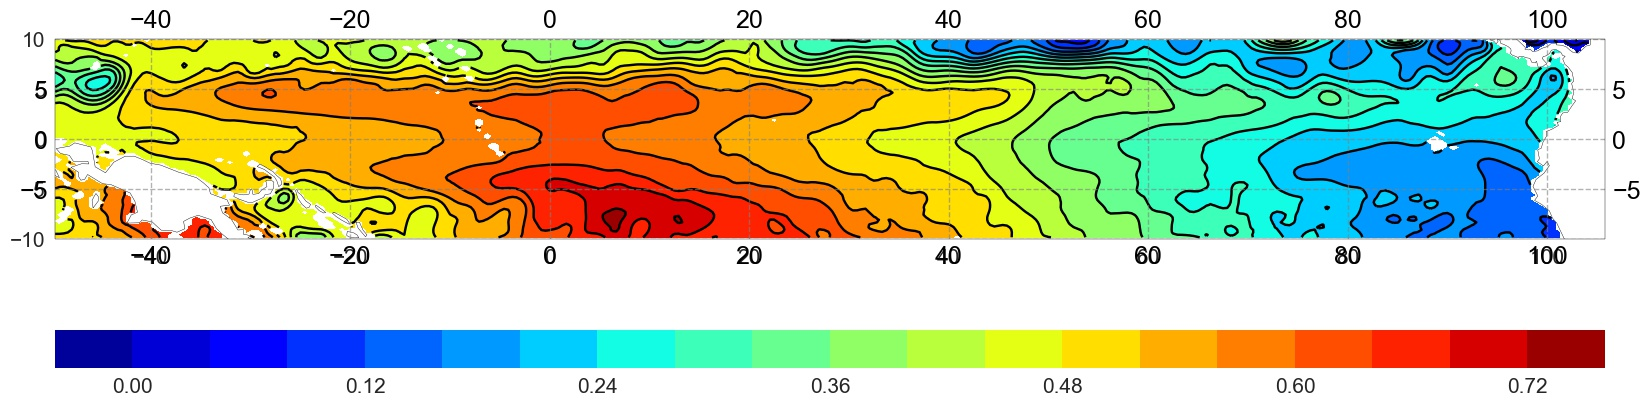
\includegraphics[width=\textwidth]{EOF.jpg}
	\caption{Modo de oscilación espacial asociado a la primer componente principal}
	\label{fig:EOF}
\end{figure}

En la estructura espacial de la EOF (Fig. \ref{fig:EOF}), puede notarse que la mayoría de las regiones en el Pacífico Este tienen un comportamiento similar, es decir, cuando una zona aumenta, la otra también lo hace. De igual forma sucede para el Pacífico Este, dónde alrededor de la piscina caliente, el nivel del mar tiene un comportamiento similar. 

La primer componente principal explica el 35\% de la varianza asociada a la banda espectral de interés, al representar la variación temporal de la estructura espacial más dominante se compara con un índice que represente la variación temporal del ENSO, en este caso, el índice ONI. Puede observarse que existe una correlación positiva, puesto que cuando hay aumentos/descensos sostenidos en el índice  ONI, la componente principal también genera sobrelevaciones/descensos en la estructura espacial, esto es similar a lo reportado previamente con la serie del mareógrafo (Fig. \ref{fig:s_d_ENSOS})

\begin{figure}[H]
	\centering
	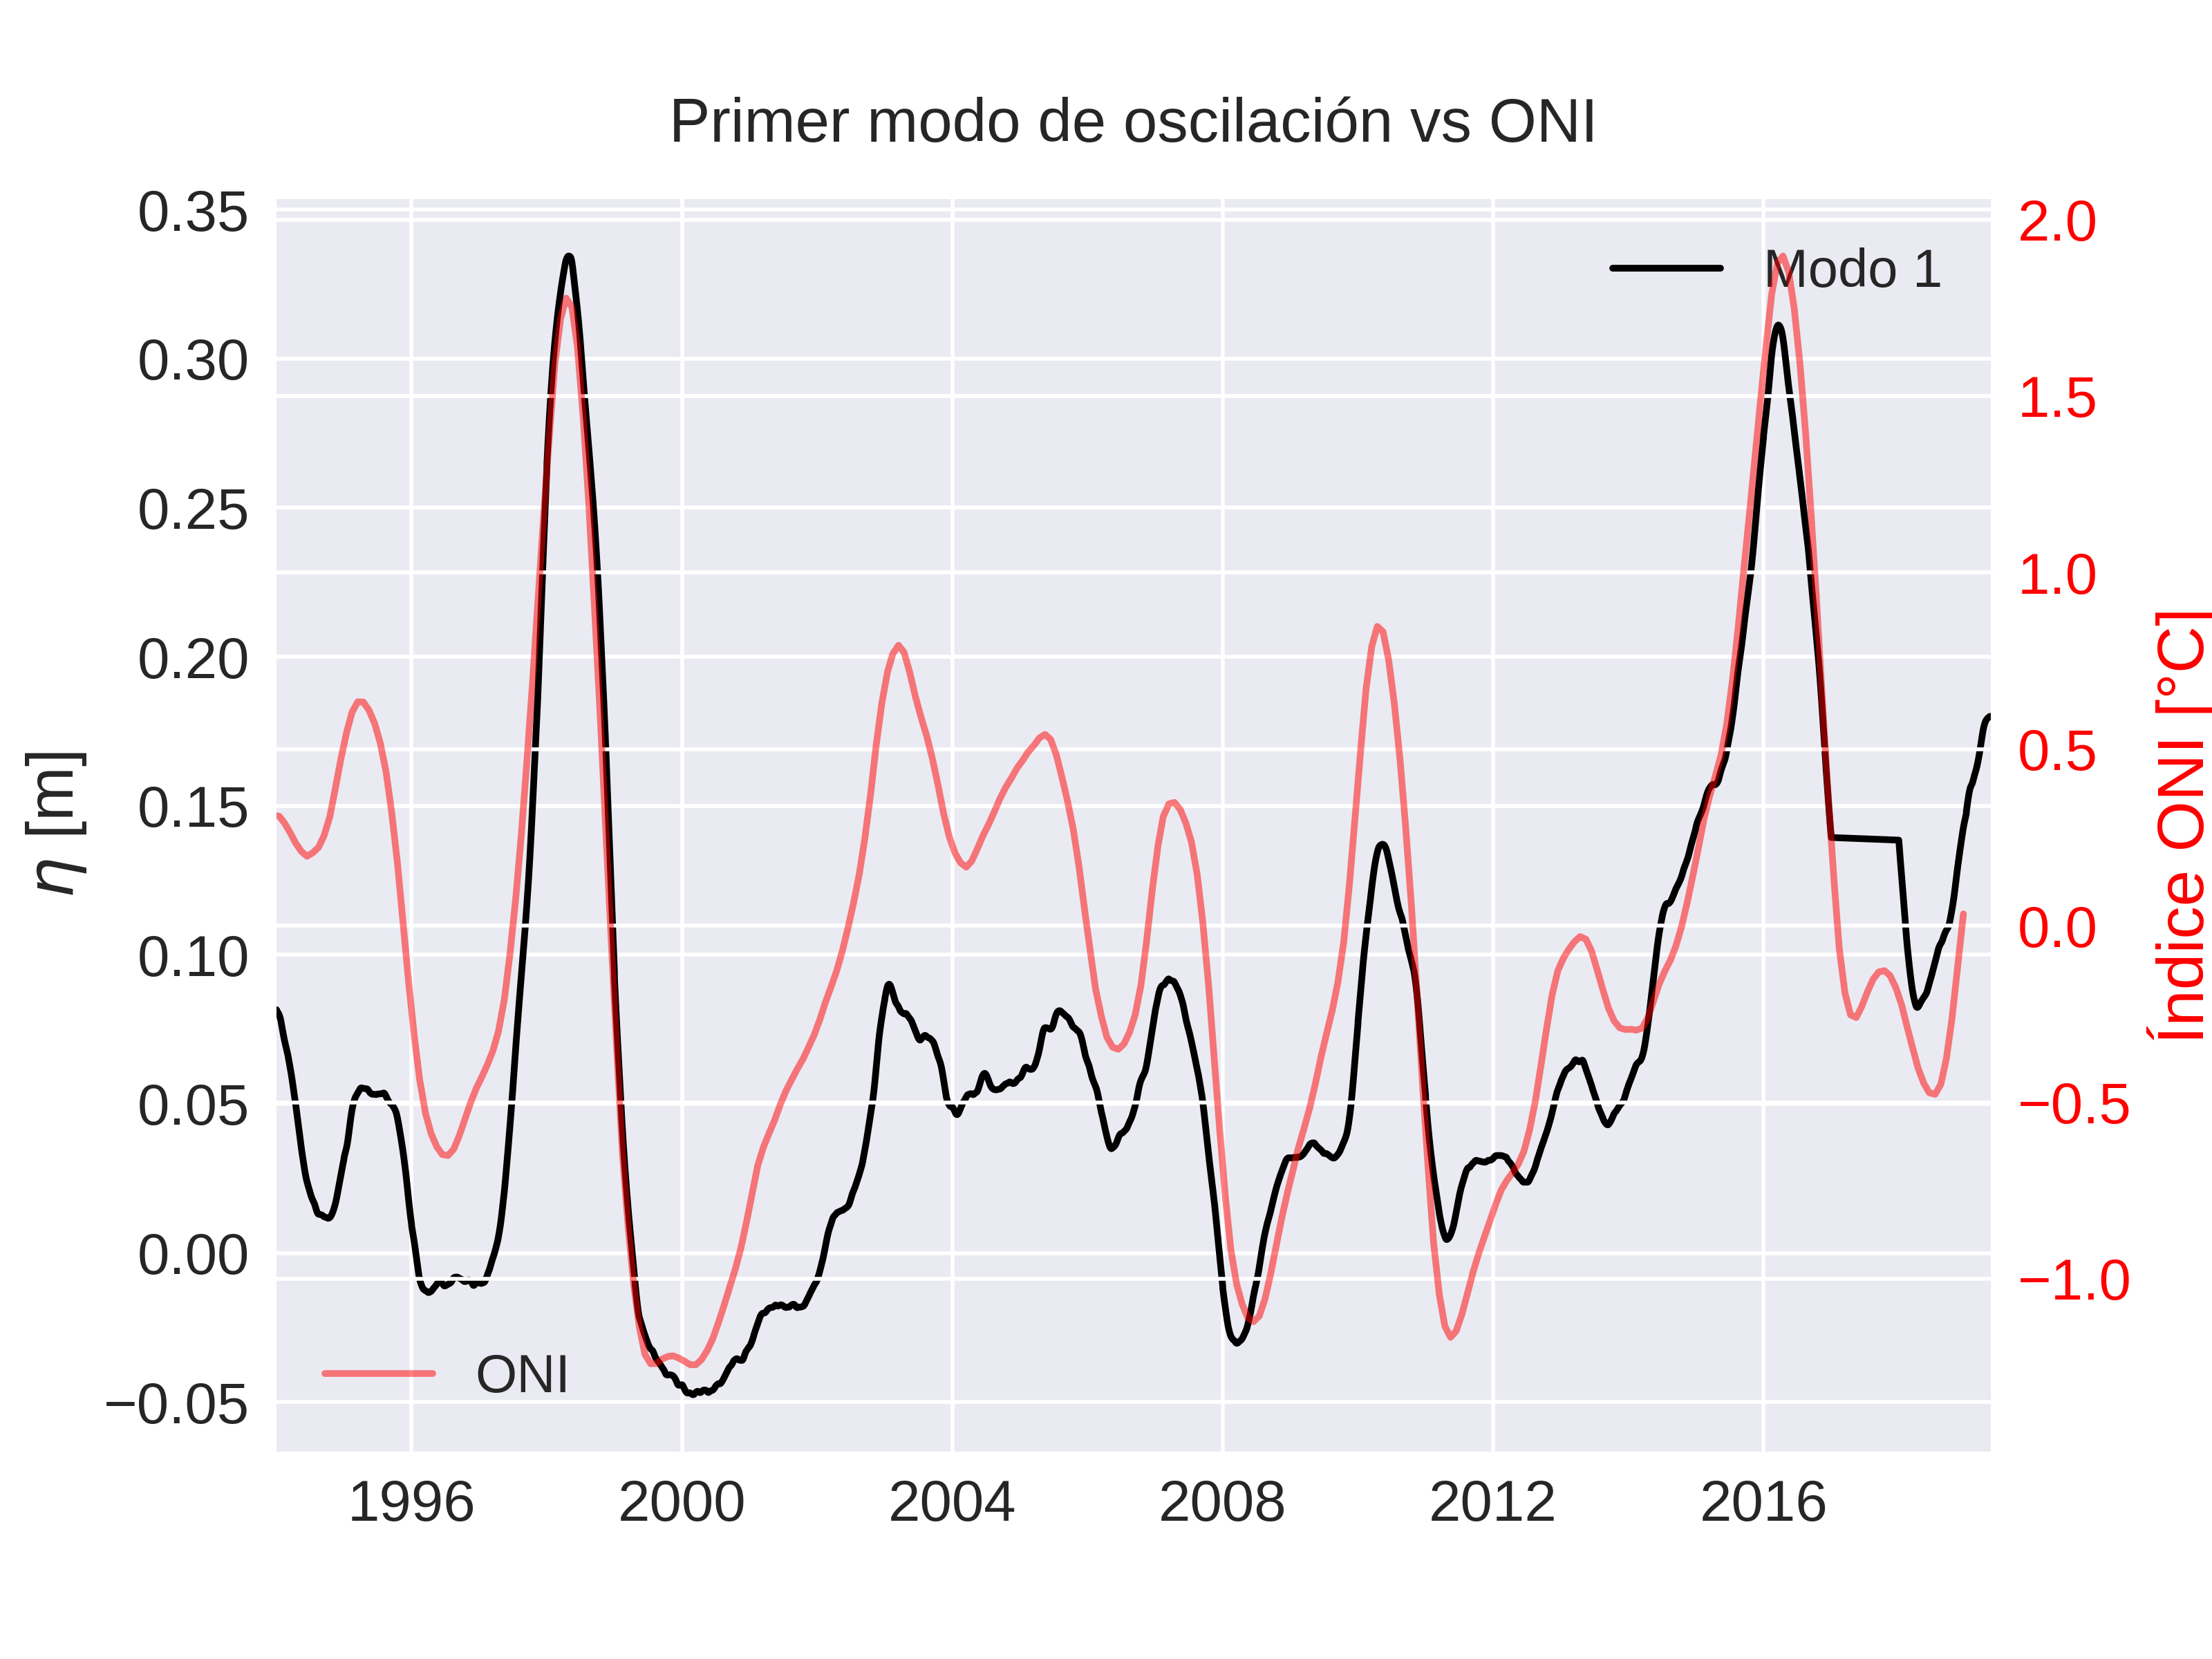
\includegraphics[scale=0.5]{mod_ONI.png}
	\caption{Comparación de la primer componente principal y el índice ONI}
	\label{fig:PC_ONI}
\end{figure}

La figura anterior sugiere que el ENSO es el patrón espacio-temporal más dominante del nivel del mar en el Pacífico Tropical para la banda frecuencial comprendida entre los 2 y 6 años, y por lo tanto, ayuda a modular las ascensos y descensos del nivel del mar en el largo plazo.

\section{Caracterización del nivel del mar durante un Evento Niño y Niña}

Es necesario un enfoque en variación espacial del nivel del mar durante eventos Niño o Niña para identificar el transporte de las sobrelevaciones y descensos que provienen desde el Oeste del Pacífico. Un diagrama de Hovmöller en la latitud 3.5$^{\circ}$N muestra como las anomalías del nivel del mar atraviesan el océano hasta llegar a la costa Pacífica Colombiana (flecha negra). Para un evento Niño se muestra que el nivel empezó aumentando hasta ciertas longitudes (cercanas a los 94$^{\circ}$W ) dónde parecieron disiparse las anomalías, pero posteriormente, aumentos aún mayores y persistentes lograron viajar mayores distancias. Lo anterior sugiere que la \textbf{persistencia} y la \textbf{intensidad} de dichas perturbaciones son factores clave para su llegada a la costa. Los valores de las anomalías son similares en magnitud a los registrados en el mareógrafo de Buenaventura (ver panel derecho en la Fig. \ref{fig:hov_nino}), adicionalmente, se vieron después de los ascensos en la costa, lo que parece ser una respuesta en forma de descensos del nivel. 

\begin{figure}[h]
	\centering
	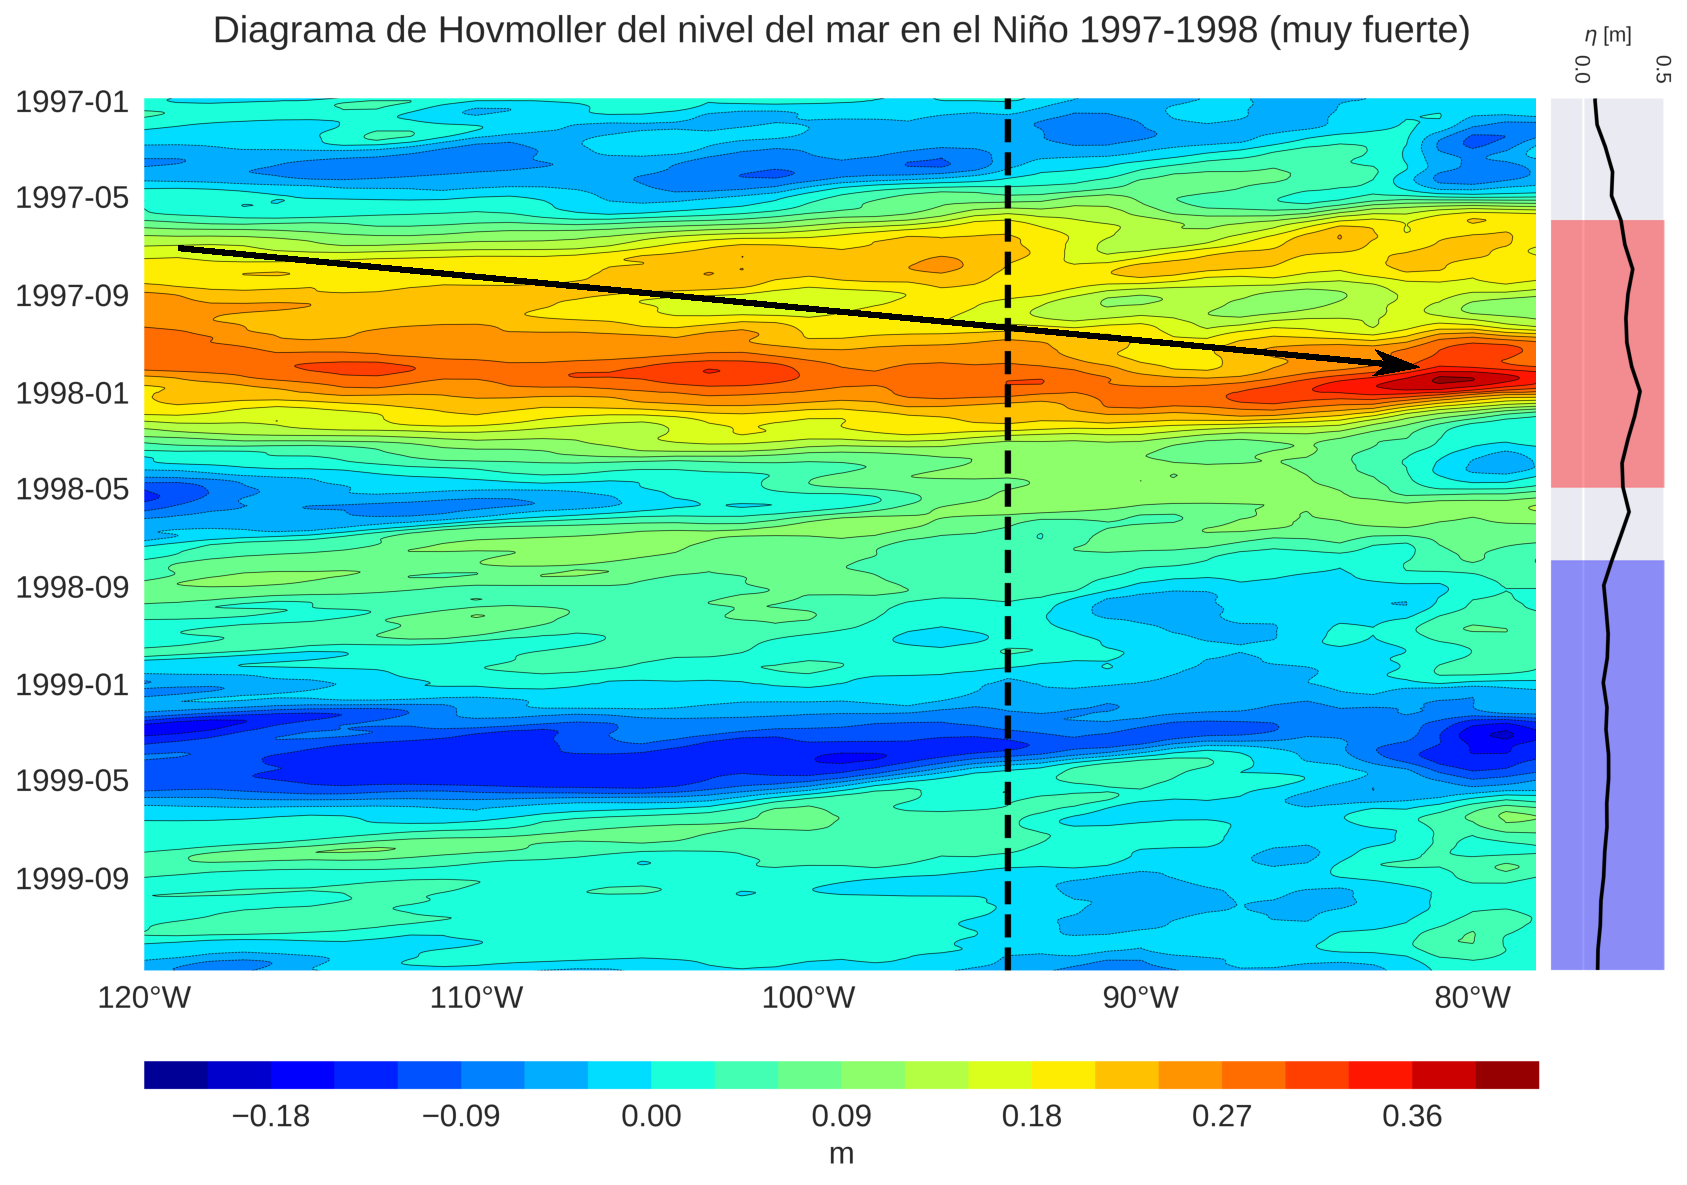
\includegraphics[width=\textwidth]{Hovmoller_nino.pdf}
	\caption{Diagrama de hovmoller en las longitudes para el nivel medio del mar durante el Niño (1997-1998)}
	\label{fig:hov_nino}
\end{figure}

Durante las fases de enfríamiento del ENSO, los vientos alisios del Este se intensifican y mantienen el centro de centro de baja presión en la piscina caliente (circulación de Walker), lo anterior, genera que el nivel del mar en el Pacífico Este disminuya. Un diagrama de Hovmoller en la latitud 3.5$^{\circ}$N muestra como las anomalías del nivel se mantienen durante un período muy largo (evento Niña de mayor duracón entre 1953 y 2010) (Fig. \ref{fig:hov_nina})

\begin{figure}[h]
	\centering
	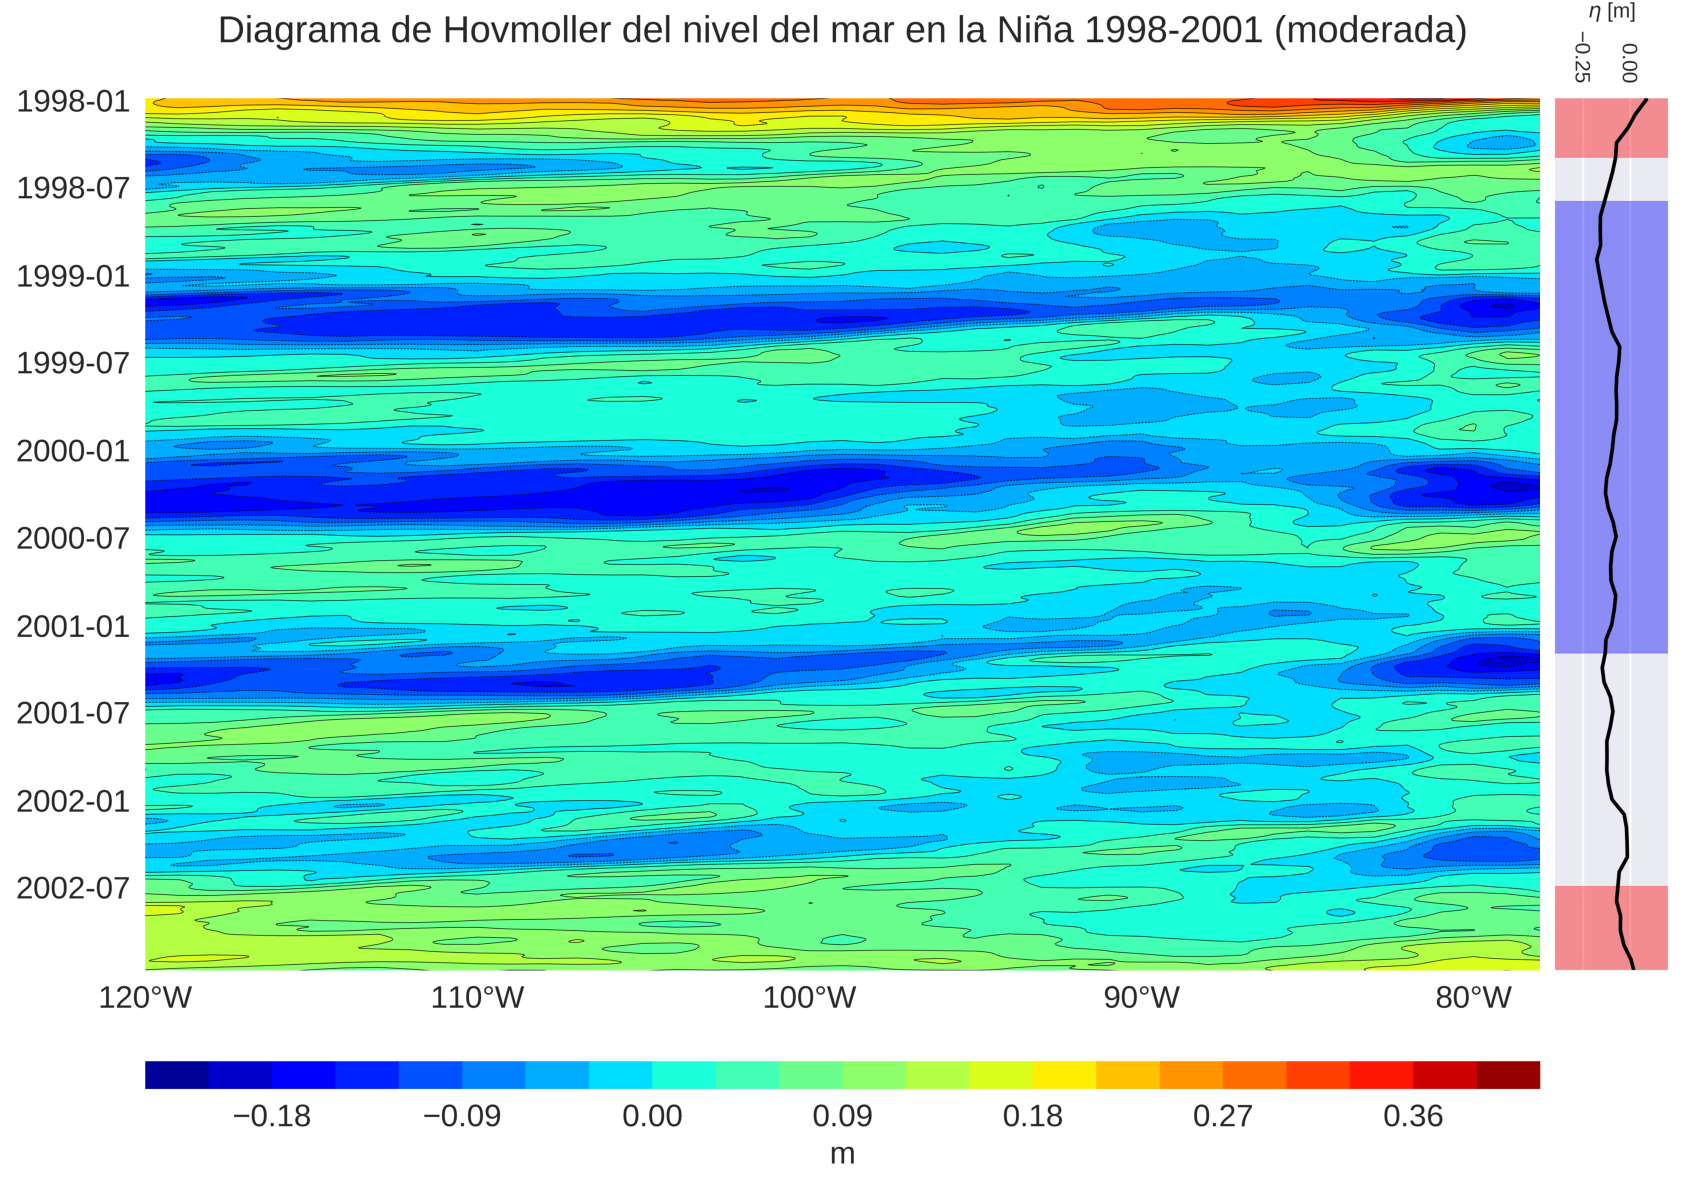
\includegraphics[width=\textwidth]{Hovmoller_nina.pdf}
	\caption{Diagrama de hovmoller en las longitudes para el nivel medio del mar durante la Niña (1998-2001)}
	\label{fig:hov_nina}
\end{figure}

El transporte de las sobrelevaciones del nivel puede indicar que hay regiones mar afuera que permiten la predicción de los aportes del nivel del mar debidos al ENSO, lo cuál sirve para generar alertas a las comunidades costeras de la bahía de Buenaventura.
%
\section{Predicción del nivel del mar debido a ENSO en una zona costera}

\subsection{Región costera de interés}

La región costera de interés seleccionada en la sección \ref{sec:1}, se muestra a junto a su respectiva serie de nivel del mar promediada espacialmente

La serie de nivel del mar se filtró en la banda de interés (Fig \ref{fig:Zona costera}), para eliminar la influencia de otros fenómenos que ocurren en escalas temporales menores (ej: ciclo anual) y mayores (ej: descongelamiento de los polos). Como se había visto previamente, en este rango de períodos existen sobrelevaciones y descensos del nivel del mar que coinciden con las franjas que marcan la ocurrencia de eventos Niño y Niña. 
%

\begin{figure}[H]
	\centering
	\subfloat[Zona costera de interés]{%
		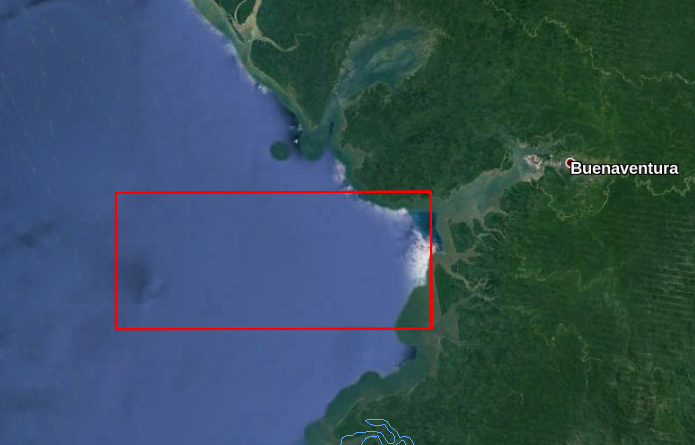
\includegraphics[scale=0.25]{zona.png}\label{subfig-1:zona}
	}
	\vspace{0.1 cm}
	\subfloat[Serie de nivel del mar representativa de la zona]{%
		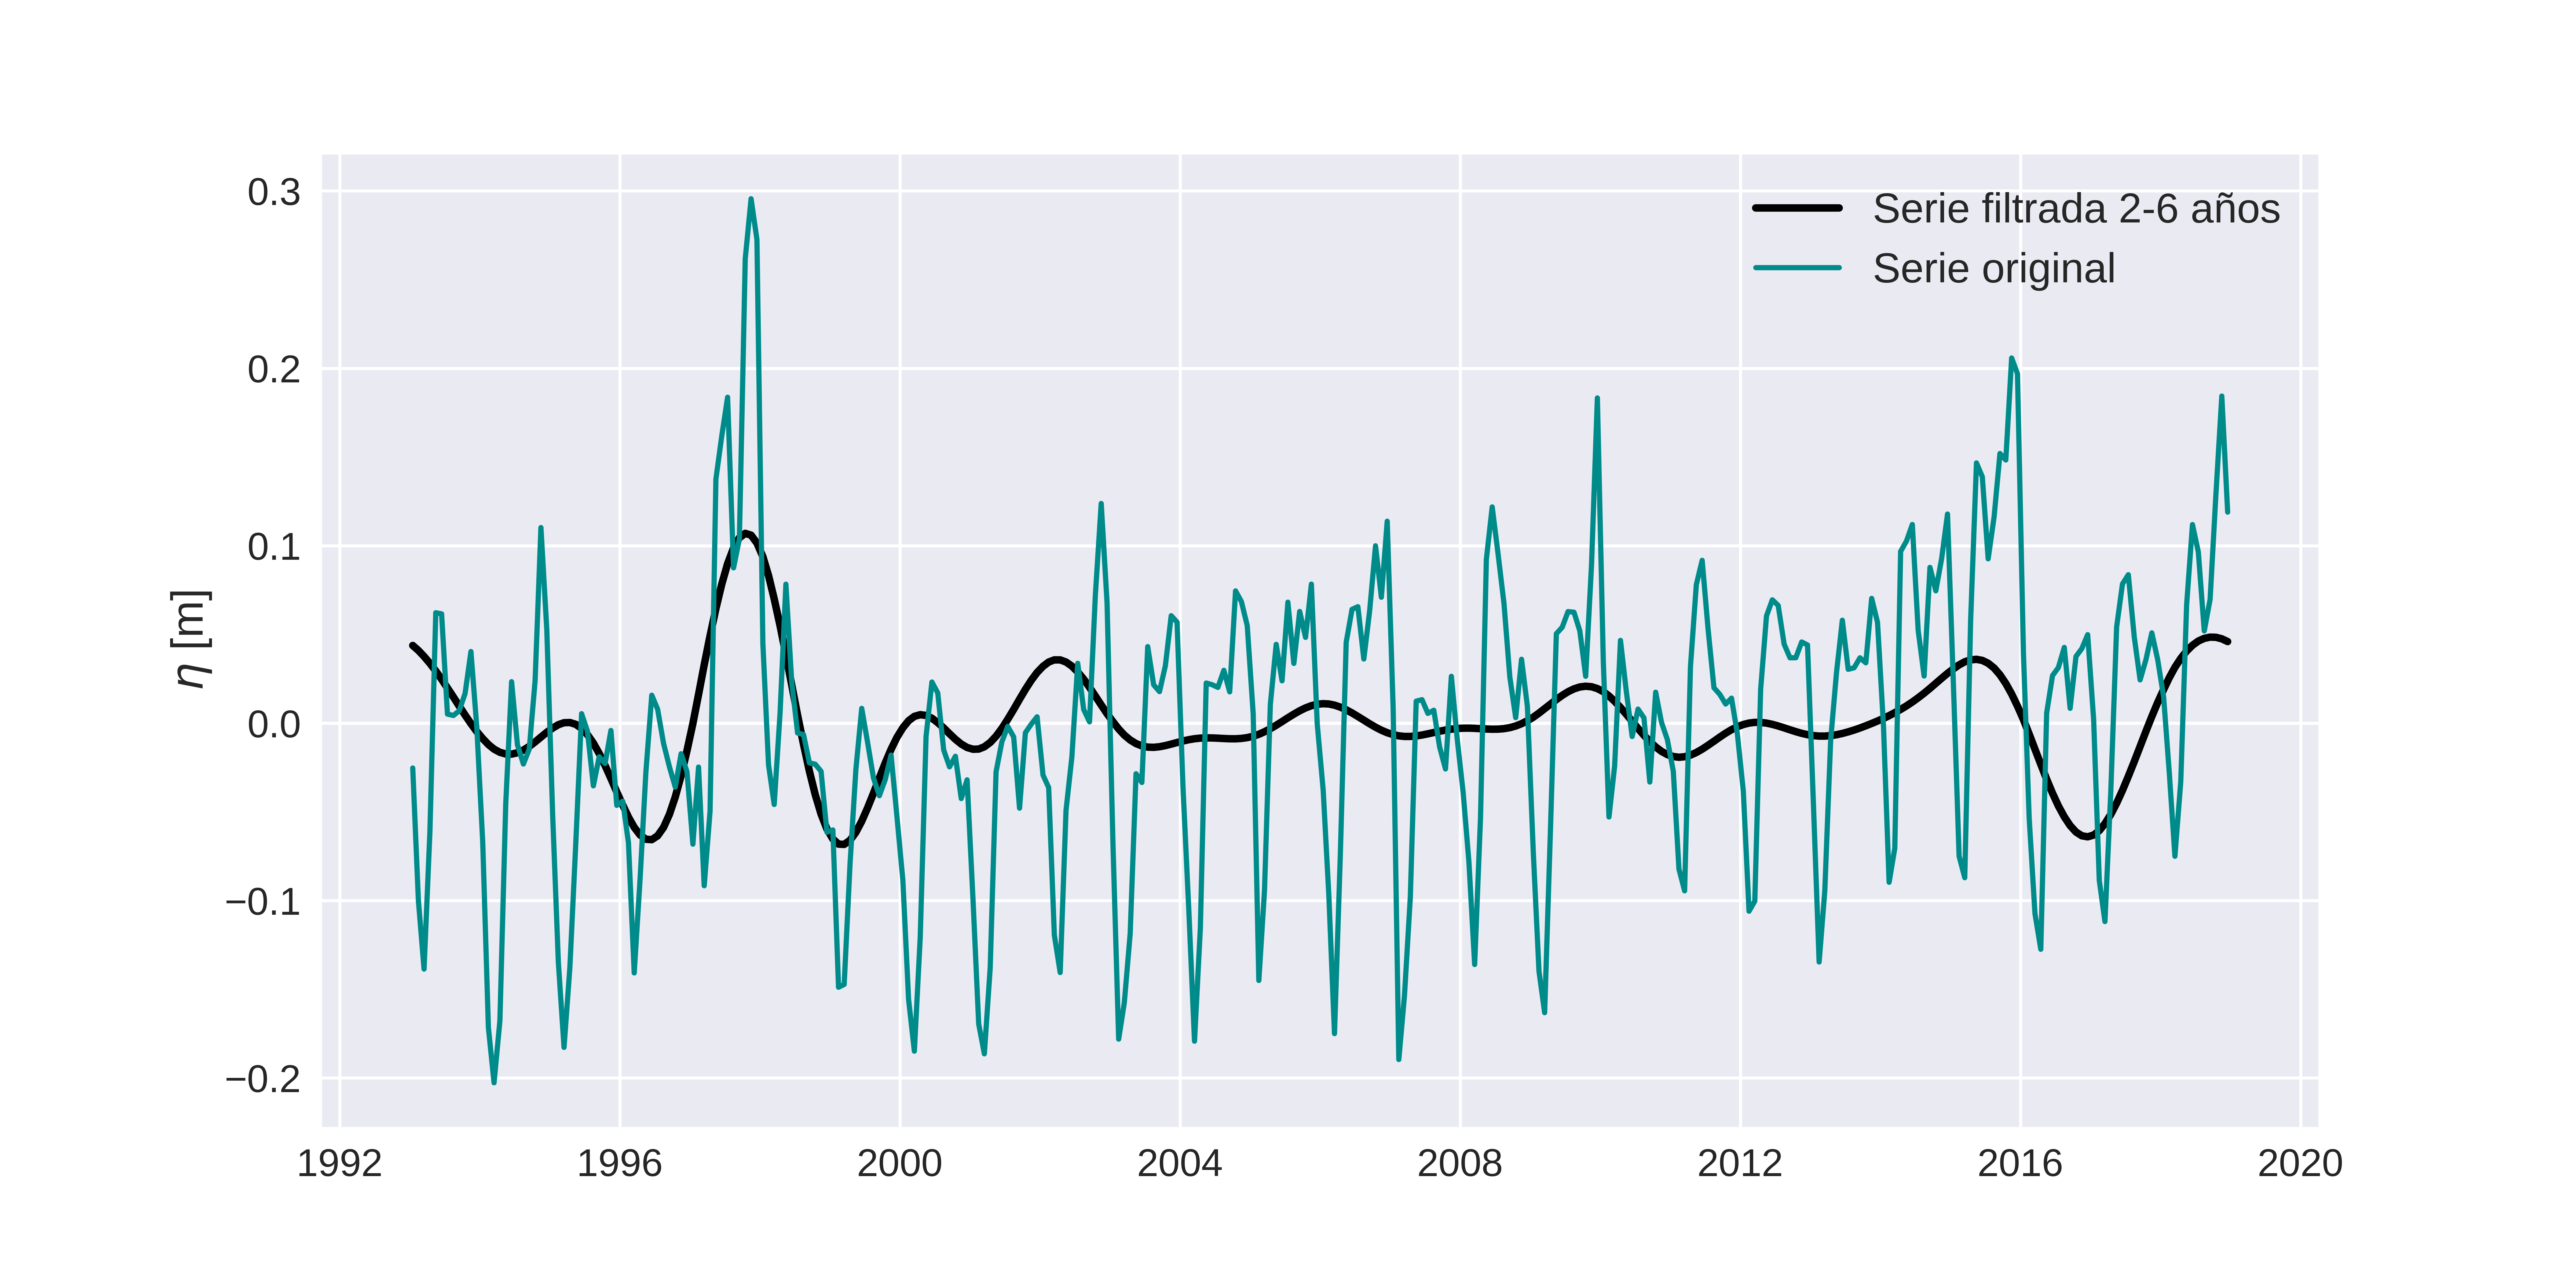
\includegraphics[scale=0.4]{serie_filtrada.png}\label{subfig-2:serie_interes}
	}
	\caption{Selección de la zona costera de interés (panel superior) y su serie representativa del nivel del mar original y filtrada entre 2 y 6 años.}
	\label{fig:Zona costera}
\end{figure}

\subsection{Selección de las regiones mar afuera }

Para predecir los aumentos y descensos del nivel del mar debidos al ENSO en la zona de interés, se determinaron regiones donde las variables de nivel del mar, temperatura y velocidad de las corrientes longitudinales y latitudinales, se correlacionan en un rezago positivo con el nivel en la costa, es decir, que mientras una variable incrementó en dicha región, el nivel del mar en la zona de interés también lo hizo un período de tiempo después. Sí existe un rezago largo, el tiempo de respuesta por parte de las comunidades costeras es mayor, sin embargo, las correlaciones disminuyen espacialmente. De todos los mapas de correlación de Spearman rezagada, se presentan los de mayor correlación en conjunto con las regiones seleccionadas para cada variable.

\begin{figure}[H]
	\subfloat[Mapa de correlación de Spearman de nivel del mar con rezago +1]{%
		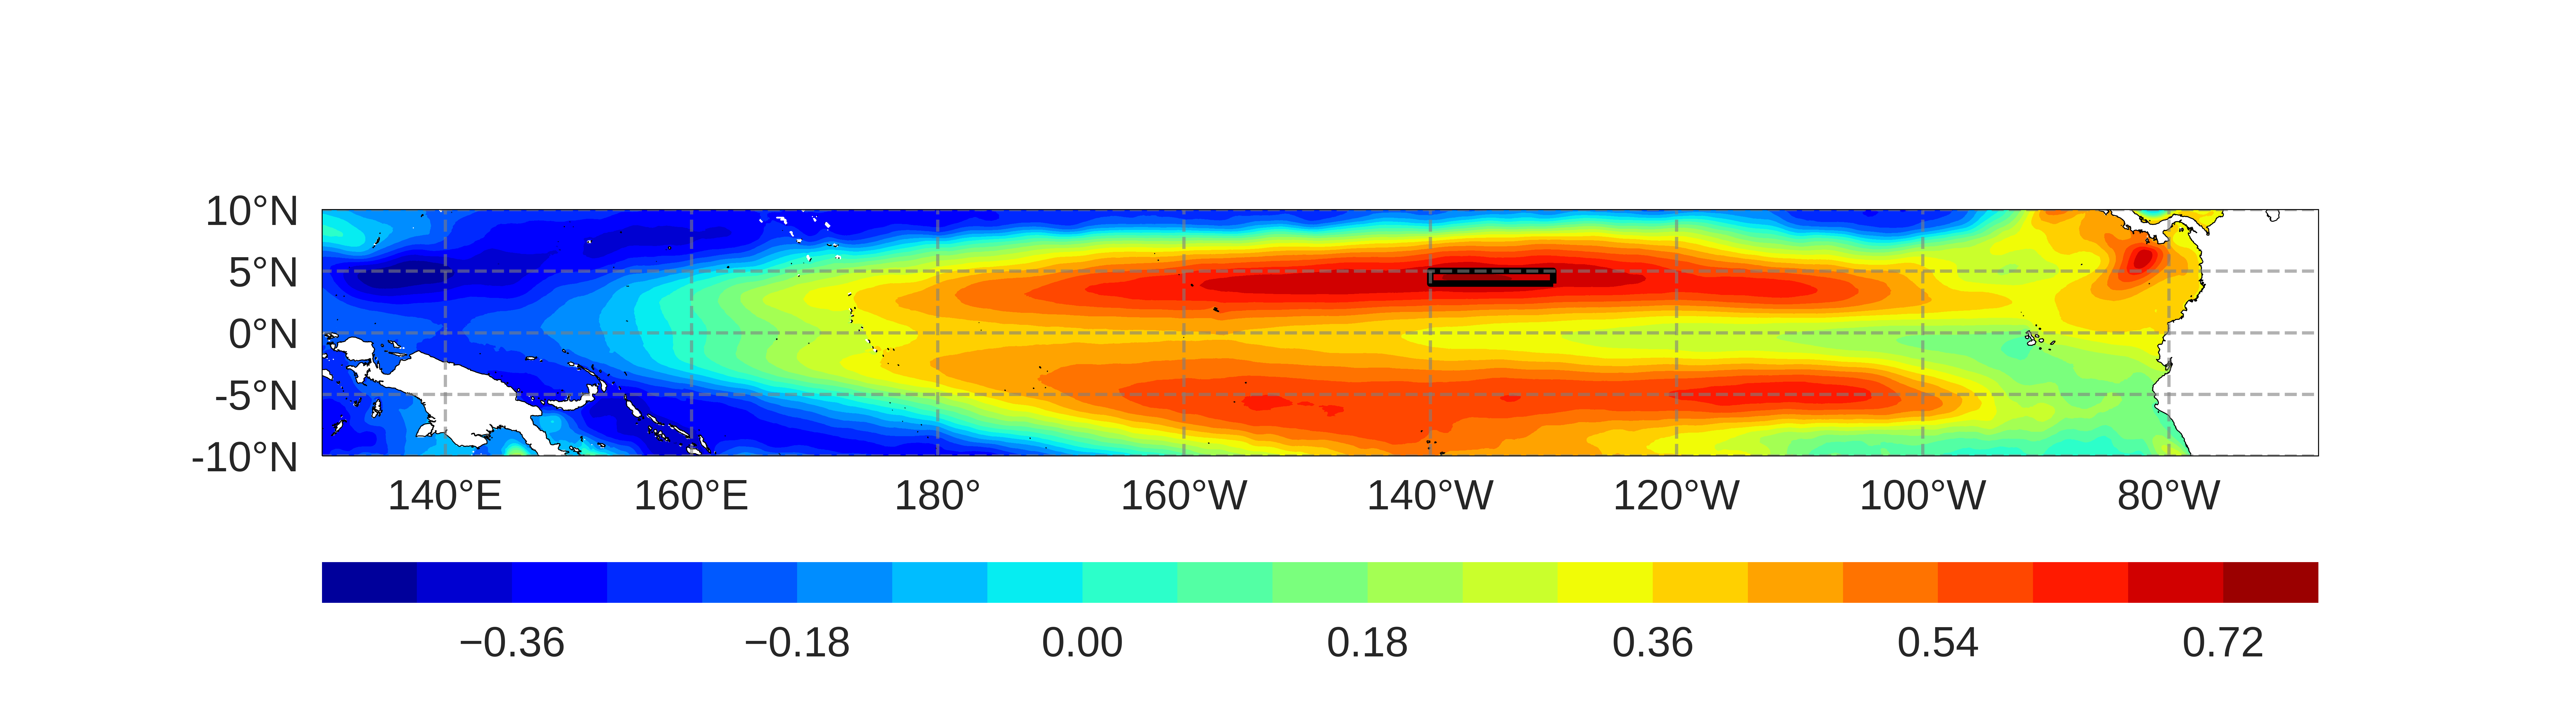
\includegraphics[width=\textwidth]{Mapa de correlacion de ssh R1_zona.png}\label{subfig-1:nmm}
	}
	\vspace{0 mm}
	\subfloat[Mapa de correlación de Spearman con rezago +1, entre el nivel del mar en la costa y la temperatura]{ 
		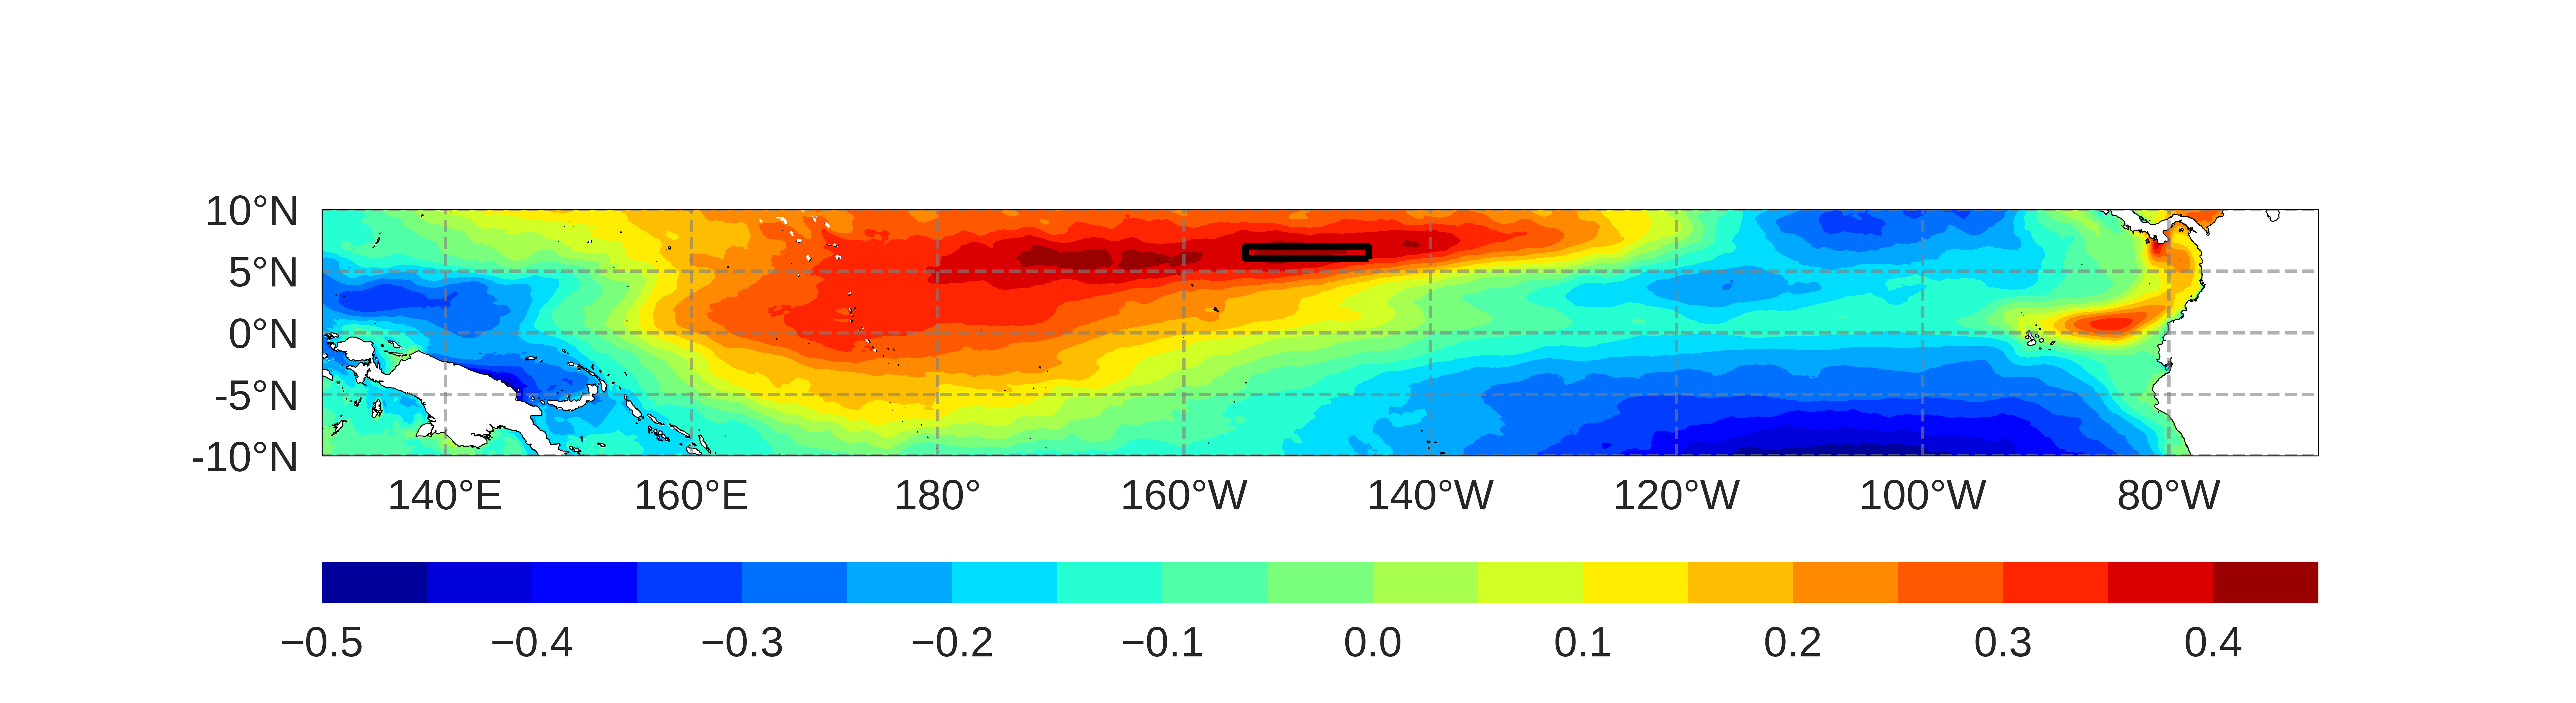
\includegraphics[width=16cm]{Mapa de correlacion de t R1_zona.png}\label{subfig-2:temp}
	}
	\newline
	\subfloat[Mapa de correlación de Spearman con rezago +1, entre el nivel del mar en la costa y la velocidad longitudinal de las corrientes superficiales ]{%
		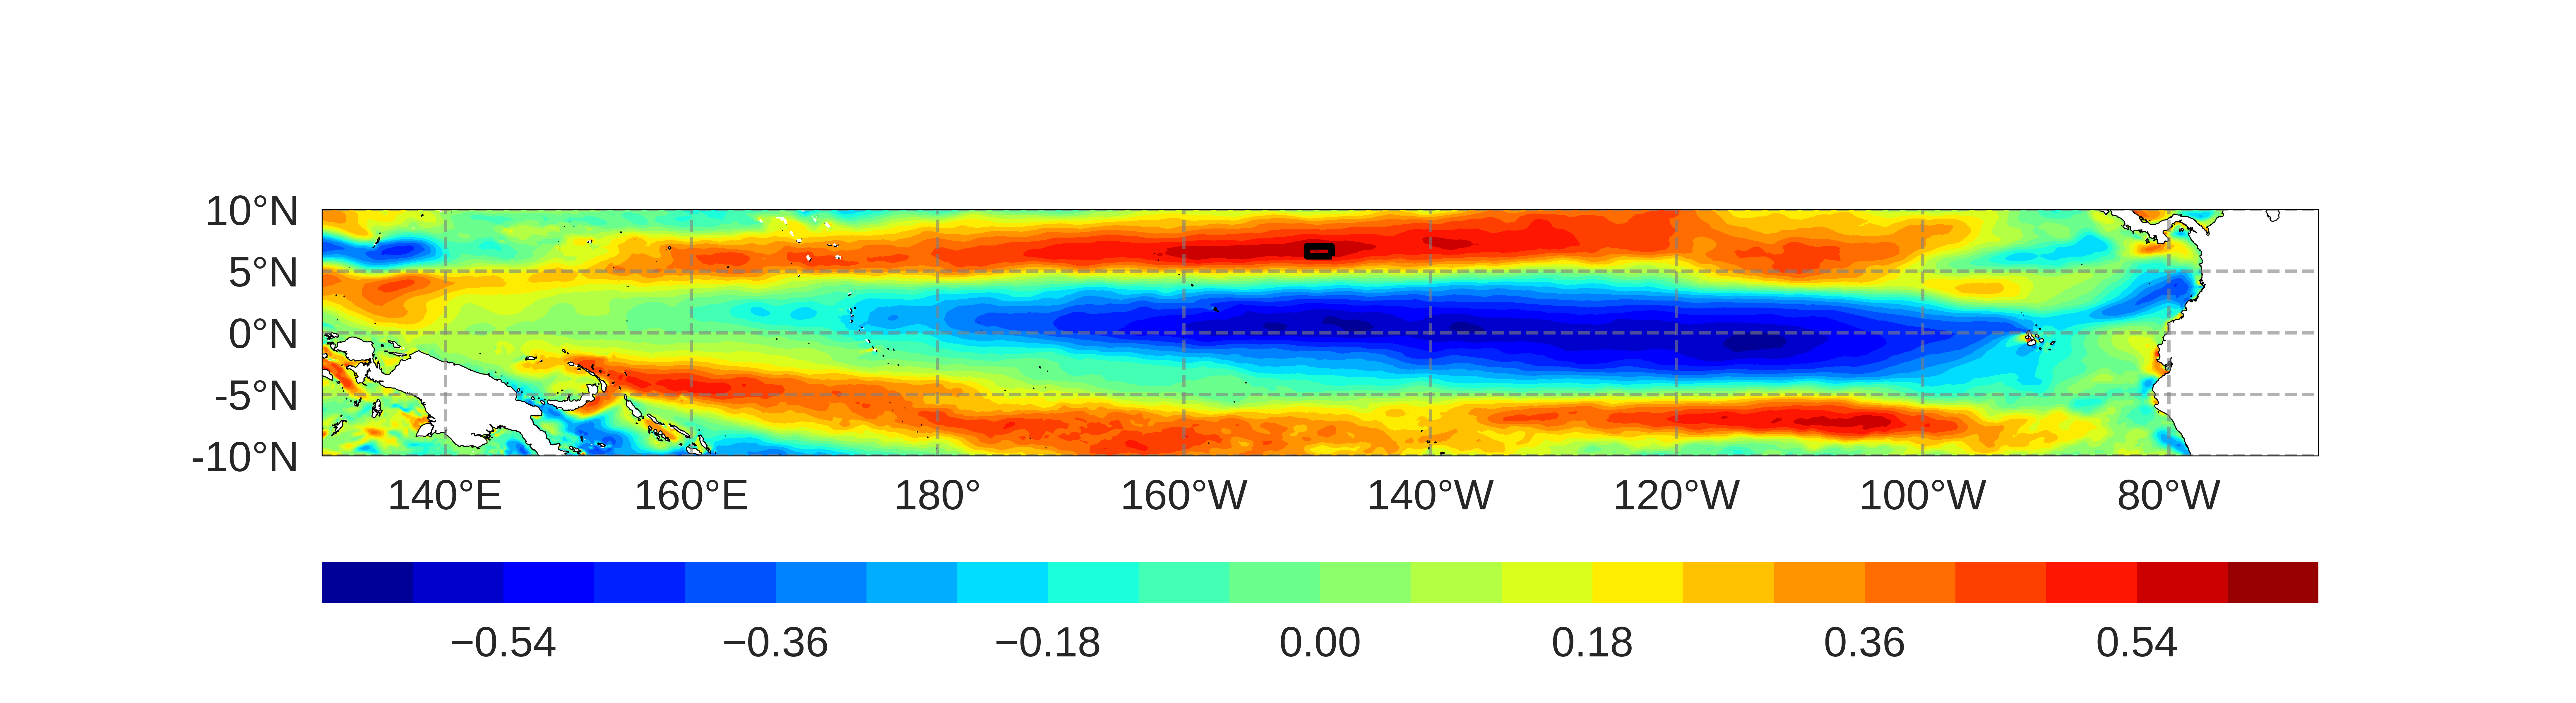
\includegraphics[width=16cm]{Mapa de correlacion de u R1_zona.png}\label{subfig-1:u}
	}
	\newpage
	\subfloat[Mapa de correlación de Spearman con rezago +1, entre el nivel del mar en la costa y la velocidad latitudinal de las corrientes superficiales]{%
		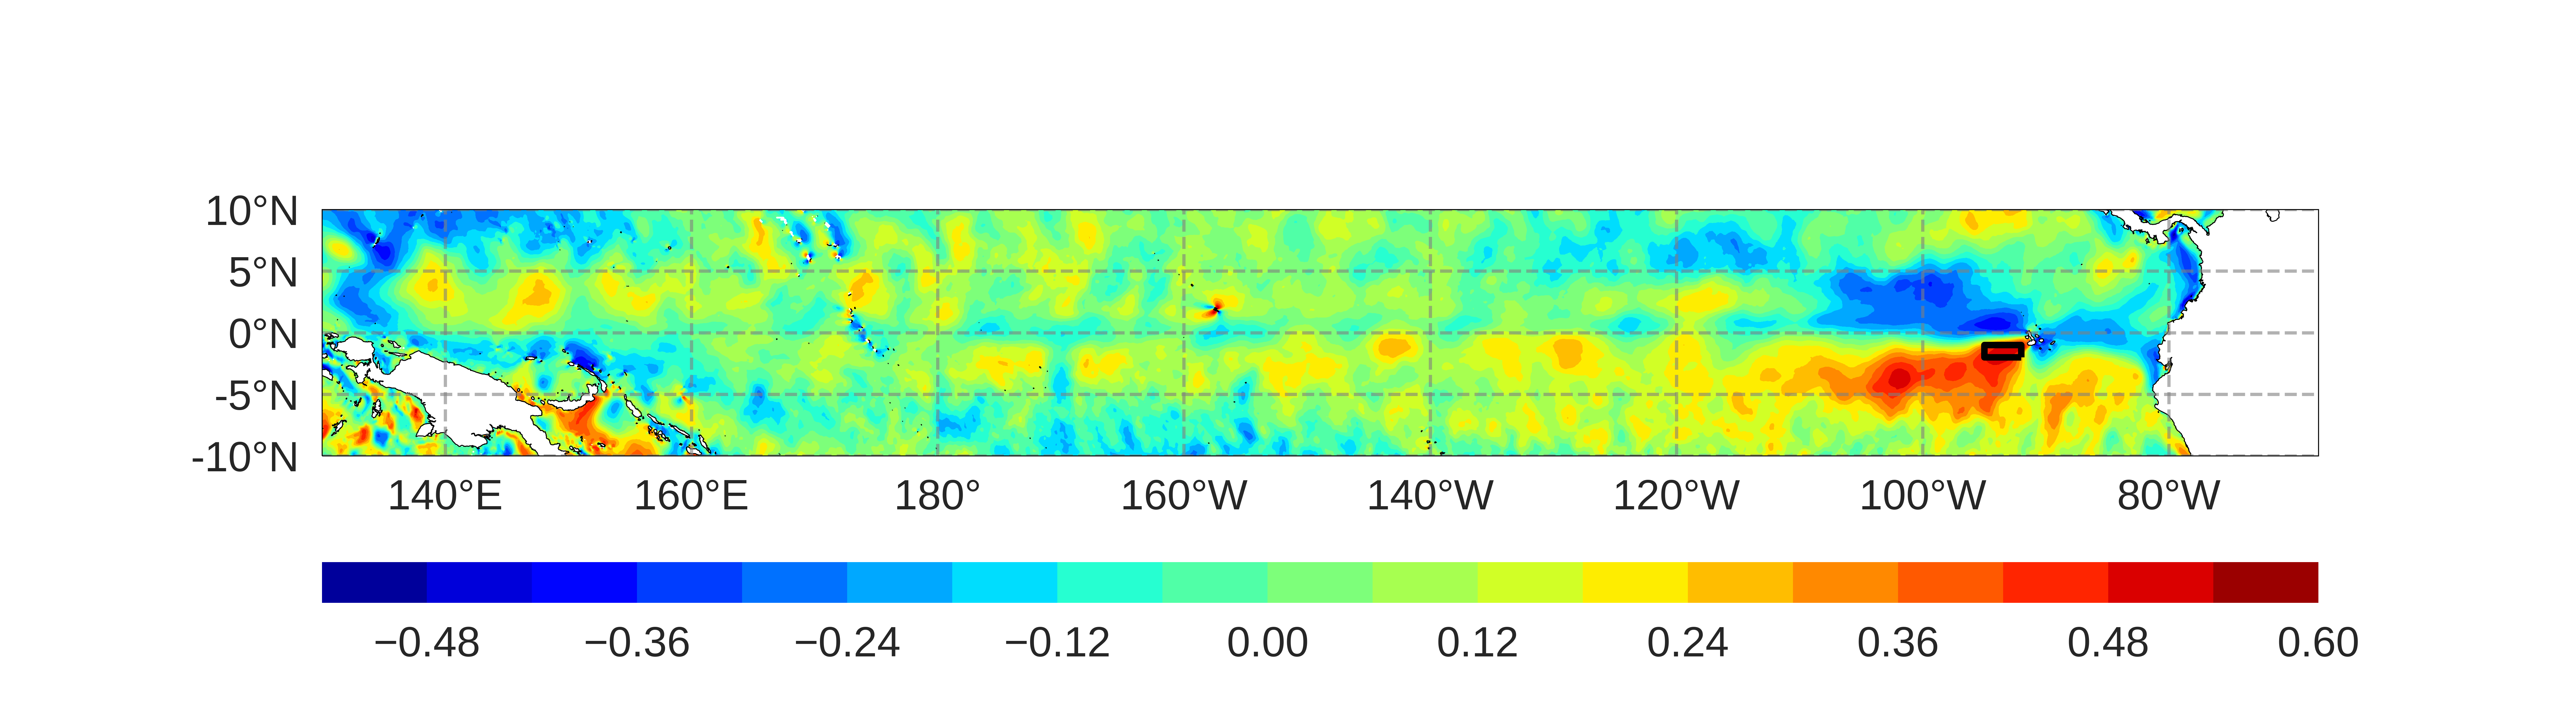
\includegraphics[width=16cm]{Mapa de correlacion de v R1_zona.png}\label{subfig-2:v}
	}
	\caption{Mapas de correlación de Spearman para todas las variables predictoras}
	\label{fig:Spearman}
\end{figure}

Las regiones seleccionadas para determinar las series de la variables que servirán como variables predictoras se presentan a continuación:

\begin{table}[H]
		\caption{Regiones elegidas para determinar las series de las variables predictoras del nivel del mar en la costa}
	\centering
	\begin{tabular}{|c|c|}
		\hline
		Variable & Región\\
		\hline		
		Nivel del mar & 4.0\textdegree N-5.0\textdegree N, 130\textdegree W - 140 \textdegree W\\
		\hline
		Temperatura & 6.\textdegree N-7.0\textdegree N, 145\textdegree W - 155\textdegree W\\
		\hline
		Velocidad de las corrientes en longitud, U & 6.7\textdegree N-4.0\textdegree N, 148\textdegree W - 150 \textdegree W\\
		\hline
		Velocidad de las corrientes en longitud, U & 1.0\textdegree S-2.0\textdegree S, 92\textdegree W- 95 \textdegree W\\
		\hline
	\end{tabular}
	\label{tab:ragions}
\end{table}

Antes de construir la red neuronal para la predicción del nivel del mar debido al fenómeno ENSO, estas series usadas de las variables \textit{predictoras} también se filtraron en la escala de interés. 

\section{Pronóstico del nivel del mar}
%
Las variables predictoras fueron pre-procesadas para optimizar las técnicas que asignan los pesos a cada unión entre nodos, este pre-procesamiento incluye el escalamiento según la función de activación. 

Después de un análisis de sensibilidad de los pesos que la red asignó a cada variable, se determinó suprimir las variables de temperatura y velocidad de las corrientes en la latitud, así se construyó la red con 2 variables de entrada, una capa oculta intermedia con dos nodos y una capa de salida con un nodo. Los pesos entre cada conexión se presentan a continuación.

\begin{figure}[H]
	\centering
	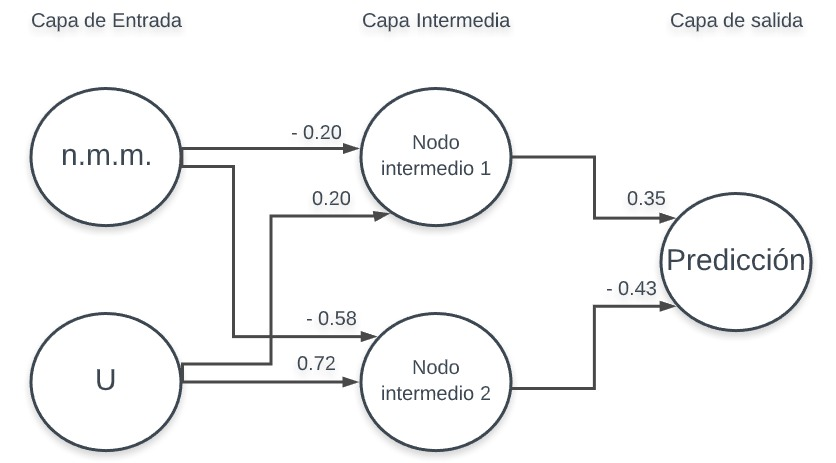
\includegraphics[scale=0.3]{Estructura de Red.jpeg}
	\caption{Estructura de la red neuronal artificial}
\end{figure}

\newpage

Después del entrenamiento de la red con el 70\% de los datos (Panel superior de la fig. \ref{fig:global_net}), la red predijo los datos de validación con un RMSE de 0.01 m y un coeficiente de correlación de Spearman igual a 0.83.

\begin{figure}[H]
\centering
\subfloat[][Comportamiento de la red neuronal artifical durante el entrenamiento ]{%
		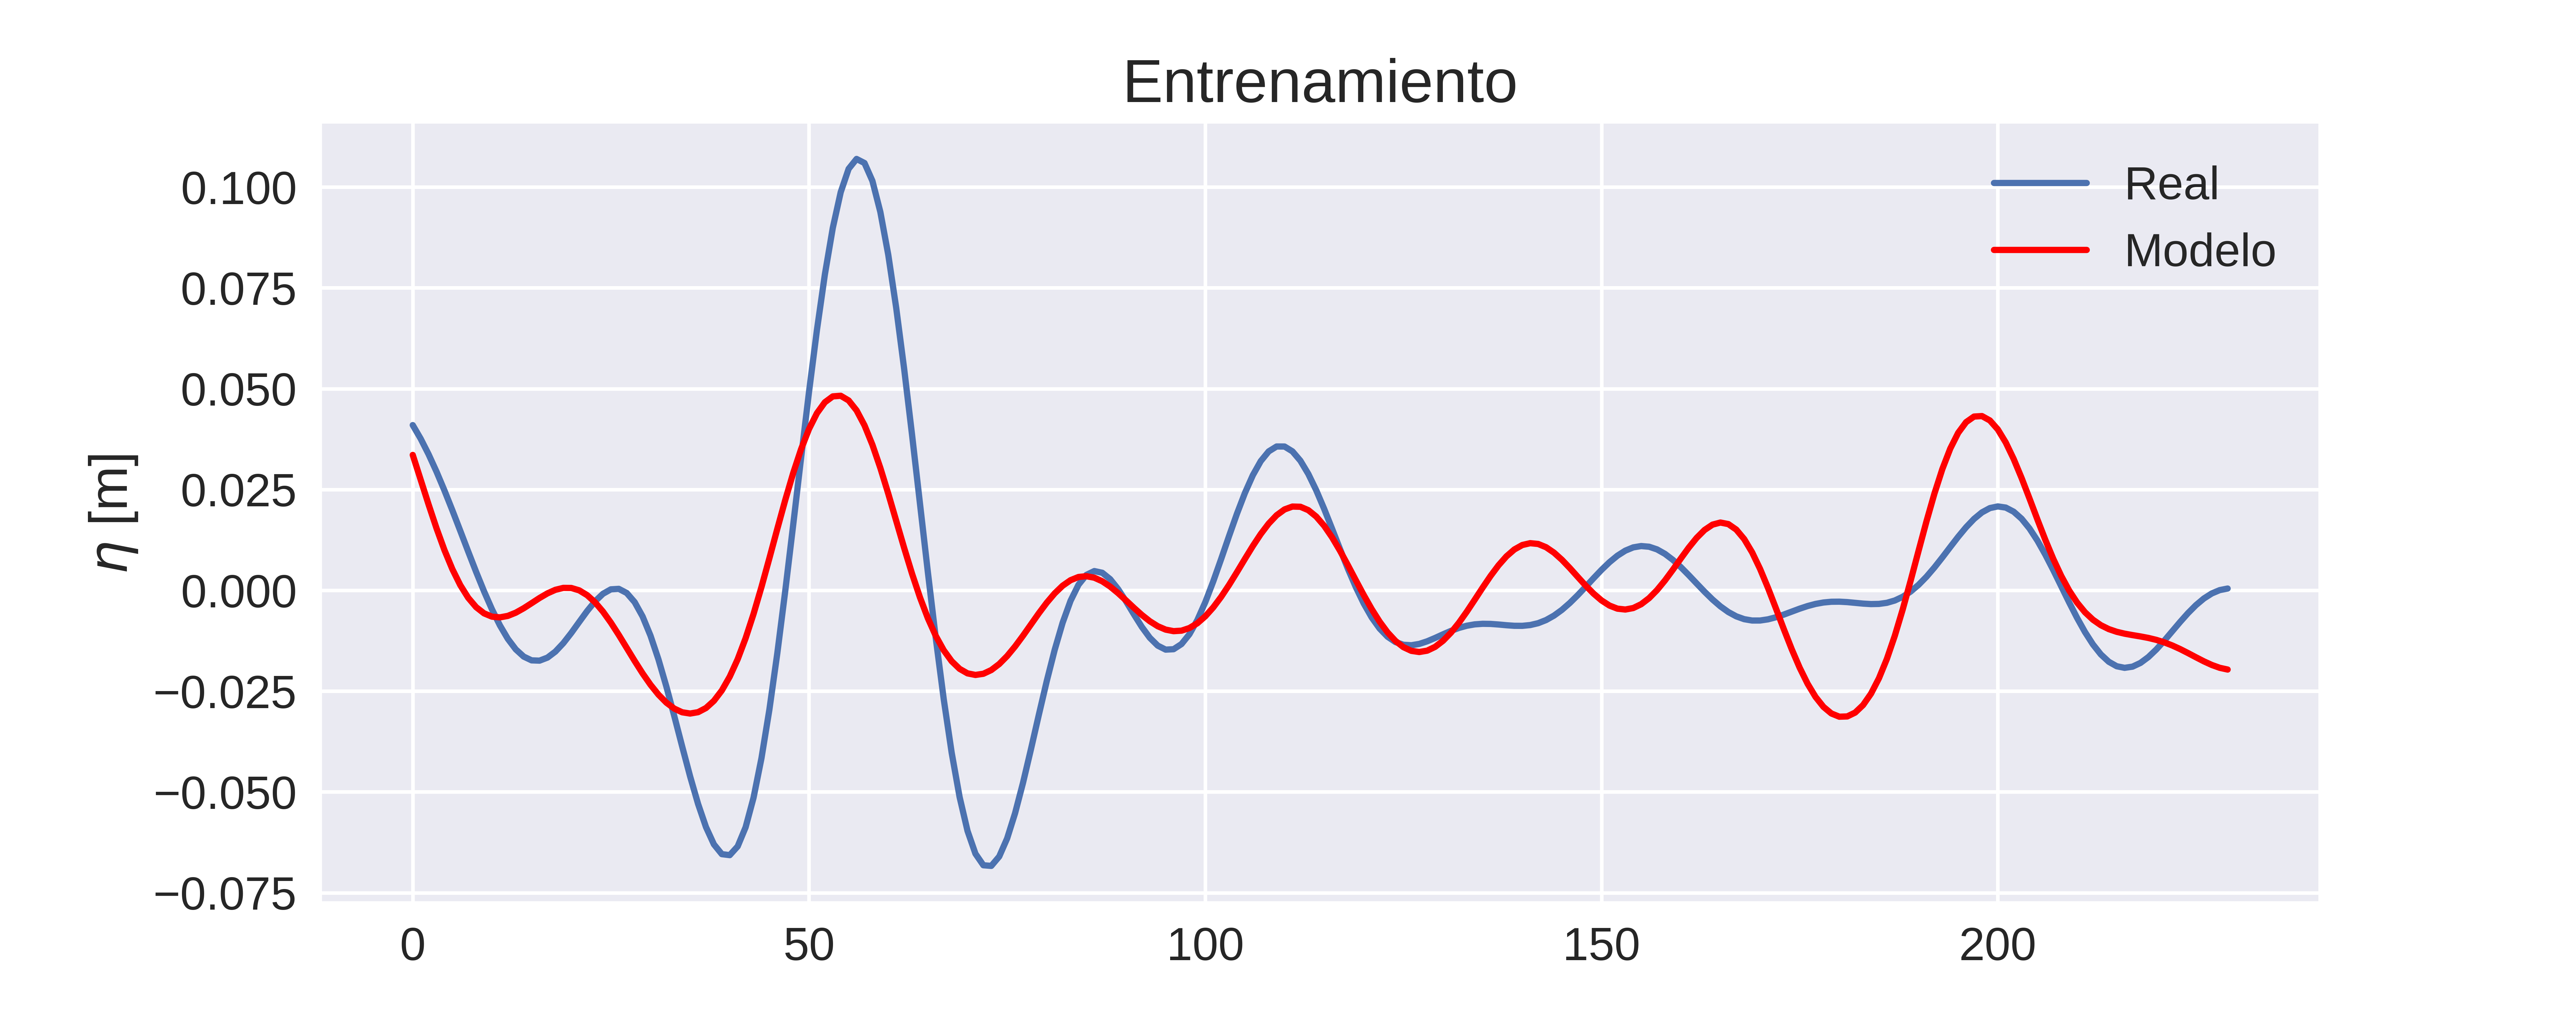
\includegraphics[scale=0.5]{red_train.png}\label{subfig-1:train}
}
\newline
\subfloat[][Predicción de los datos de validación con la red neuronal artificial]{%
	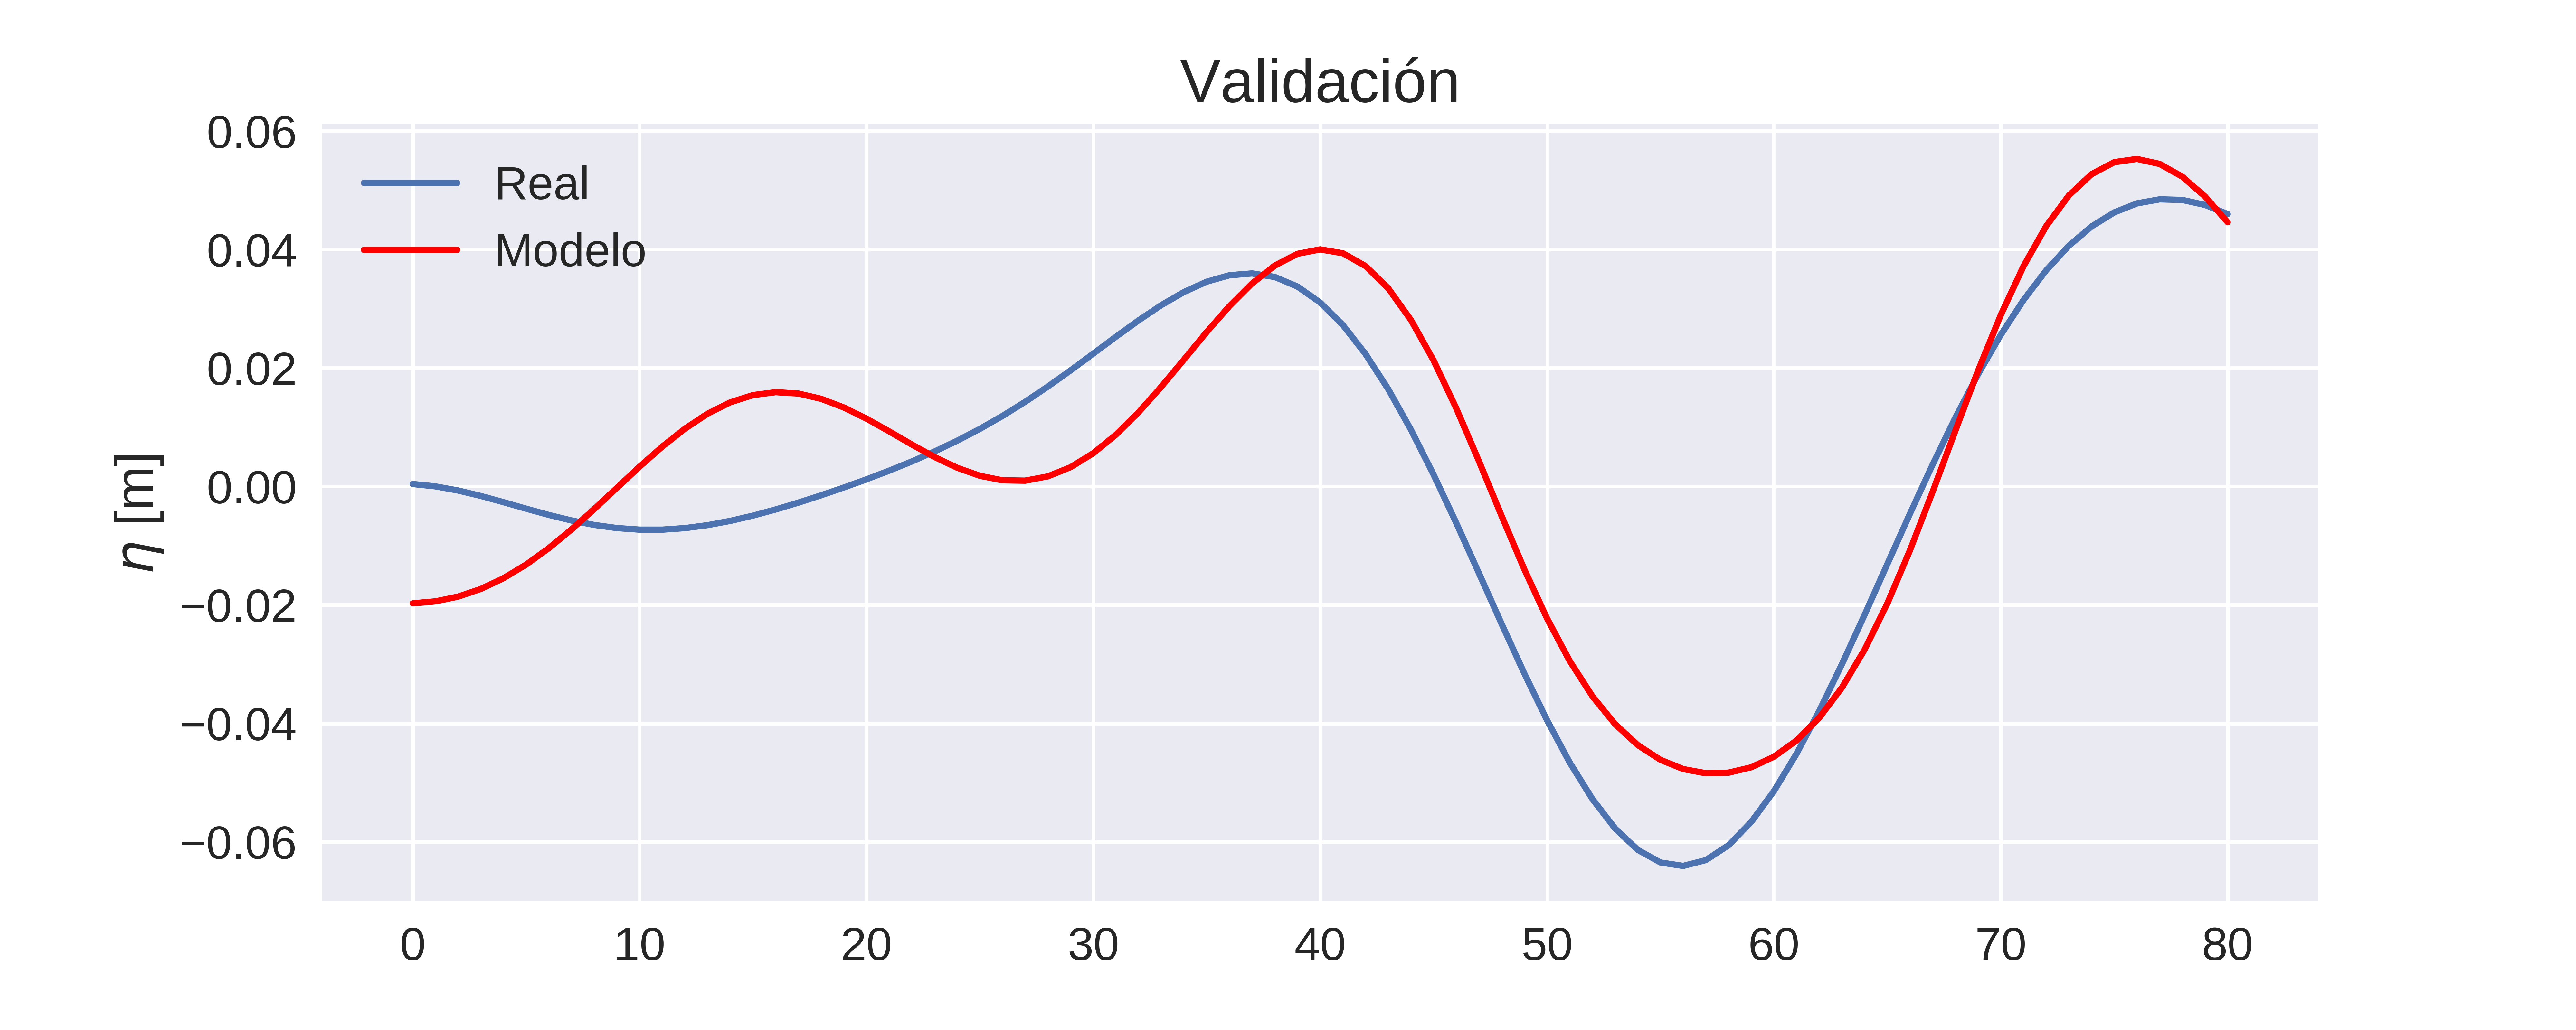
\includegraphics[scale=0.5]{red_test.png}\label{subfig-2:test}
}
\caption{Comportamiento de la red en el entrenamiento y en la validación}
\label{fig:global_net}
\end{figure}
%
%
%
%
%
%
